%%
%% Beginning of file 'sample61.tex'
%%
%% Modified 2016 September
%%
%% This is a sample manuscript marked up using the
%% AASTeX v6.1 LaTeX 2e macros.
%%
%% AASTeX is now based on Alexey Vikhlinin's emulateapj.cls 
%% (Copyright 2000-2015).  See the classfile for details.

%% AASTeX requires revtex4-1.cls (http://publish.aps.org/revtex4/) and
%% other external packages (latexsym, graphicx, amssymb, longtable, and epsf).
%% All of these external packages should already be present in the modern TeX 
%% distributions.  If not they can also be obtained at www.ctan.org.

%% The first piece of markup in an AASTeX v6.x document is the \documentclass
%% command. LaTeX will ignore any data that comes before this command. The 
%% documentclass can take an optional argument to modify the output style.
%% The command below calls the preprint style  which will produce a tightly 
%% typeset, one-column, single-spaced document.  It is the default and thus
%% does not need to be explicitly stated.
%%
%%
%% using aastex version 6.1
\documentclass[twocolumn]{aastex62}

%% The default is a single spaced, 10 point font, single spaced article.
%% There are 5 other style options available via an optional argument. They
%% can be envoked like this:
%%
%% \documentclass[argument]{aastex61}
%% 
%% where the arguement options are:
%%
%%  twocolumn   : two text columns, 10 point font, single spaced article.
%%                This is the most compact and represent the final published
%%                derived PDF copy of the accepted manuscript from the publisher
%%  manuscript  : one text column, 12 point font, double spaced article.
%%  preprint    : one text column, 12 point font, single spaced article.  
%%  preprint2   : two text columns, 12 point font, single spaced article.
%%  modern      : a stylish, single text column, 12 point font, article with
%% 		  wider left and right margins. This uses the Daniel
%% 		  Foreman-Mackey and David Hogg design.
%%
%% Note that you can submit to the AAS Journals in any of these 6 styles.
%%
%% There are other optional arguments one can envoke to allow other stylistic
%% actions. The available options are:
%%
%%  astrosymb    : Loads Astrosymb font and define \astrocommands. 
%%  tighten      : Makes baselineskip slightly smaller, only works with 
%%                 the twocolumn substyle.
%%  times        : uses times font instead of the default
%%  linenumbers  : turn on lineno package.
%%  trackchanges : required to see the revision mark up and print its output
%%  longauthor   : Do not use the more compressed footnote style (default) for 
%%                 the author/collaboration/affiliations. Instead print all
%%                 affiliation information after each name. Creates a much
%%                 long author list but may be desirable for short author papers
%%
%% these can be used in any combination, e.g.
%%
%% \documentclass[twocolumn,linenumbers,trackchanges]{aastex61}

%% AASTeX v6.* now includes \hyperref support. While we have built in specific
%% defaults into the classfile you can manually override them with the
%% \hypersetup command. For example,
%%
%%\hypersetup{linkcolor=red,citecolor=green,filecolor=cyan,urlcolor=magenta}
%%
%% will change the color of the internal links to red, the links to the
%% bibliography to green, the file links to cyan, and the external links to
%% magenta. Additional information on \hyperref options can be found here:
%% https://www.tug.org/applications/hyperref/manual.html#x1-40003

%% If you want to create your own macros, you can do so
%% using \newcommand. Your macros should appear before
%% the \begin{document} command.
%%
\usepackage{multirow, amsmath}
\newcommand{\vdag}{(v)^\dagger}
\newcommand\aastex{AAS\TeX}
\newcommand\latex{La\TeX}
\newcommand{\sm}{M_\odot}
\newcommand{\sr}{R_\odot}

%% Reintroduced the \received and \accepted commands from AASTeX v5.2
\received{\today}
\revised{}
\accepted{}
%% Command to document which AAS Journal the manuscript was submitted to.
%% Adds "Submitted to " the arguement.
\submitjournal{PASP}

%% Mark up commands to limit the number of authors on the front page.
%% Note that in AASTeX v6.1 a \collaboration call (see below) counts as
%% an author in this case.
%
%\AuthorCollaborationLimit=3
%
%% Will only show Schwarz, Muench and "the AAS Journals Data Scientist 
%% collaboration" on the front page of this example manuscript.
%%
%% Note that all of the author will be shown in the published article.
%% This feature is meant to be used prior to acceptance to make the
%% front end of a long author article more manageable. Please do not use
%% this functionality for manuscripts with less than 20 authors. Conversely,
%% please do use this when the number of authors exceeds 40.
%%
%% Use \allauthors at the manuscript end to show the full author list.
%% This command should only be used with \AuthorCollaborationLimit is used.

%% The following command can be used to set the latex table counters.  It
%% is needed in this document because it uses a mix of latex tabular and
%% AASTeX deluxetables.  In general it should not be needed.
%\setcounter{table}{1}

%%%%%%%%%%%%%%%%%%%%%%%%%%%%%%%%%%%%%%%%%%%%%%%%%%%%%%%%%%%%%%%%%%%%%%%%%%%%%%%%
%%
%% The following section outlines numerous optional output that
%% can be displayed in the front matter or as running meta-data.
%%
%% If you wish, you may supply running head information, although
%% this information may be modified by the editorial offices.
\shorttitle{PS1 Star-galaxy Catalog}
\shortauthors{One then the other}
%%
%% You can add a light gray and diagonal water-mark to the first page 
%% with this command:
\watermark{DRAFT}
%% where "text", e.g. DRAFT, is the text to appear.  If the text is 
%% long you can control the water-mark size with:
%  \setwatermarkfontsize{dimension}
%% where dimension is any recognized LaTeX dimension, e.g. pt, in, etc.
%%
%%%%%%%%%%%%%%%%%%%%%%%%%%%%%%%%%%%%%%%%%%%%%%%%%%%%%%%%%%%%%%%%%%%%%%%%%%%%%%%%

%%%%%%%%%%%%%%%%%%%%%%%%%%%%%%%%%%%%%%%%%%%%%%%%%%%%%%%%%%%%%%%%%%%%%%%%%%%%%%%%
%%
%% The following section defines new commands for comments from co-authors
%%
\newcommand{\yutaro}[1]{{\color{red} yt: {#1}}}
\newcommand{\NC}[1]{{\color{brown} NC: {#1}}}
\newcommand{\aam}[1]{{\color{blue} aam: {#1}}}
\newcommand{\todo}[1]{{\color{magenta} to-do: {#1}}}
%%
%%%%%%%%%%%%%%%%%%%%%%%%%%%%%%%%%%%%%%%%%%%%%%%%%%%%%%%%%%%%%%%%%%%%%%%%%%%%%%%%

%% This is the end of the preamble.  Indicate the beginning of the
%% manuscript itself with \begin{document}.

\begin{document}

\title{A PanSTARRS1 Star--Galaxy Separation Model: \\
       Application in the ZTF Real-Time Pipeline
       }

%% LaTeX will automatically break titles if they run longer than
%% one line. However, you may use \\ to force a line break if
%% you desire. In v6.1 you can include a footnote in the title.

%% A significant change from earlier AASTEX versions is in the structure for 
%% calling author and affilations. The change was necessary to implement 
%% autoindexing of affilations which prior was a manual process that could 
%% easily be tedious in large author manuscripts.
%%
%% The \author command is the same as before except it now takes an optional
%% arguement which is the 16 digit ORCID. The syntax is:
%% \author[xxxx-xxxx-xxxx-xxxx]{Author Name}
%%
%% This will hyperlink the author name to the author's ORCID page. Note that
%% during compilation, LaTeX will do some limited checking of the format of
%% the ID to make sure it is valid.
%%
%% Use \affiliation for affiliation information. The old \affil is now aliased
%% to \affiliation. AASTeX v6.1 will automatically index these in the header.
%% When a duplicate is found its index will be the same as its previous entry.
%%
%% Note that \altaffilmark and \altaffiltext have been removed and thus 
%% can not be used to document secondary affiliations. If they are used latex
%% will issue a specific error message and quit. Please use multiple 
%% \affiliation calls for to document more than one affiliation.
%%
%% The new \altaffiliation can be used to indicate some secondary information
%% such as fellowships. This command produces a non-numeric footnote that is
%% set away from the numeric \affiliation footnotes.  NOTE that if an
%% \altaffiliation command is used it must come BEFORE the \affiliation call,
%% right after the \author command, in order to place the footnotes in
%% the proper location.
%%
%% Use \email to set provide email addresses. Each \email will appear on its
%% own line so you can put multiple email address in one \email call. A new
%% \correspondingauthor command is available in V6.1 to identify the
%% corresponding author of the manuscript. It is the author's responsibility
%% to make sure this name is also in the author list.
%%
%% While authors can be grouped inside the same \author and \affiliation
%% commands it is better to have a single author for each. This allows for
%% one to exploit all the new benefits and should make book-keeping easier.
%%
%% If done correctly the peer review system will be able to
%% automatically put the author and affiliation information from the manuscript
%% and save the corresponding author the trouble of entering it by hand.

\correspondingauthor{Yutaro Tachibana}
\email{tachibana@hp.phys.titech.ac.jp}


\author[0000-0001-6584-6945]{Yutaro Tachibana}
\affil{Department of Physics, Tokyo Institute of Technology, 2-12-1 Ookayama, Meguro-ku, Tokyo 152-8551,
Japan}
\affil{Department of Physics, Math, and Astronomy, California Institute of Technology, Pasadena, CA, 91125}

\author[0000-0001-9515-478X]{A.~A.~Miller}
\affil{Center for Interdisciplinary Exploration and Research in Astrophysics (CIERA) and Department of Physics and Astronomy, Northwestern University, 2145 Sheridan Road, Evanston, IL 60208, USA}
\affil{The Adler Planetarium, Chicago, IL 60605, USA}


%% Note that the \and command from previous versions of AASTeX is now
%% depreciated in this version as it is no longer necessary. AASTeX 
%% automatically takes care of all commas and "and"s between authors names.

%% AASTeX 6.1 has the new \collaboration and \nocollaboration commands to
%% provide the collaboration status of a group of authors. These commands 
%% can be used either before or after the list of corresponding authors. The
%% argument for \collaboration is the collaboration identifier. Authors are
%% encouraged to surround collaboration identifiers with ()s. The 
%% \nocollaboration command takes no argument and exists to indicate that
%% the nearby authors are not part of surrounding collaborations.

%% Mark off the abstract in the ``abstract'' environment. 
\begin{abstract}

In the era of large photometric surveys, the importance of automated and
accurate classification is rapidly increasing. Specifically, the separation
of stars and galaxies in astronomical imaging is a critical initial step for
a wide array of studies, ranging from Galactic science to large scale
structure and cosmology. Here, we present our method to construct a large,
deep catalog of stars and galaxies utilizing Pan-STARRS1 (PS1) 3$\pi$ survey
data, which consists of $\sim$3$\times10^9$ sources with
$m\lesssim23.5$\,mag. We develop a supervised machine-learning methodology,
using the random forest (RF) algorithm, to construct the PS1 star--galaxy
separation model. We train the model using $\sim$5$\times10^4$ PS1 sources
with \textit{HST} COSMOS morphological classifications and assess its
performance using $\sim$4$\times10^6$ sources with Sloan Digital Sky Survey
(SDSS) spectra. We construct 11 ``white flux'' features, which combine PS1
flux and shape measurements across 5 filters, to increase the signal-to-noise
ratio relative to any individual filter. The RF model is compared to 3
alternative models, including the SDSS and PS1 photometric classification
models, and we find that the RF model performs best. By number the PS1
catalog is dominated by faint sources ($m\gtrsim21$\,mag), and in this regime
the RF model significantly outperforms the SDSS and PS1 models. For
time-domain surveys, star--galaxy separation is crucial for identifying the
Galactic or extragalactic origin of new transients. We have classified
$\sim$1.5$\times10^9$ sources using the RF model, and these results are used
within the Zwicky Transient Facility real-time pipeline to automatically
reject stellar sources from the extragalactic alert stream.

\end{abstract}

%% Keywords should appear after the \end{abstract} command. 
%% See the online documentation for the full list of available subject
%% keywords and the rules for their use.
\keywords{catalogs --- galaxies: statistics --- methods: data analysis --- methods: statistical --- stars: statistics --- surveys}

%% From the front matter, we move on to the body of the paper.
%% Sections are demarcated by \section and \subsection, respectively.
%% Observe the use of the LaTeX \label
%% command after the \subsection to give a symbolic KEY to the
%% subsection for cross-referencing in a \ref command.
%% You can use LaTeX's \ref and \label commands to keep track of
%% cross-references to sections, equations, tables, and figures.
%% That way, if you change the order of any elements, LaTeX will
%% automatically renumber them.

%% We recommend that authors also use the natbib \citep
%% and \citet commands to identify citations.  The citations are
%% tied to the reference list via symbolic KEYs. The KEY corresponds
%% to the KEY in the \bibitem in the reference list below. 

\section{Introduction}\label{sec:intro}

The proliferation of wide-field optical detectors has led to a plethora of
imaging catalogs in the past two decades. Separating unresolved point sources (i.e., stars and quasi-stellar objects
[QSOs]) from photometrically extended sources (i.e., galaxies) is one of the
most challenging and important steps in the extraction of astronomical
information from these imaging catalogs. For faint sources especially,
performing this task well boosts our progress in understanding the Universe 
\NC{
(e.g., \citealt{Sevilla18}).
}
The high fidelity separation of stars and galaxies allows us to investigate
the nature of dark matter by: (i) tracing structure in the Milky Way halo
(e.g., \citealt{Belokurov06}), (ii) measuring galaxy-galaxy correlation
functions (e.g., \citealt{Ross11, Ho15}), and (iii) detecting the weak
lensing signal from cosmic shear \citep{Soumagnac15}. Complete, and pure,
catalogs of galaxies can be used to assess the the geometry of the Universe
\citep{Yasuda01} and the theory of galaxy formation (e.g.,
\citealt{Loveday12, Moorman15}). Finally, for time-domain surveys,
star--galaxy catalogs enable an immediate classification for all newly
discovered variable phenomena as being either Galatic or extragalactic in
origin (e.g., \citealt{Berger12,Miller17}).

Given the many applications for a catalog that separates point sources from
galaxies, we turn our attention to the Pan-STARRS1 (PS1) 3$\pi$ survey
\citep{Chambers16}, whose $\sim$3$\times 10^{9}$ source catalog provides a
felicitous data set.

The 1.8\,m PS1 telescope is equipped with a wide-field ($\sim$7\,deg$^2$)
1.4 gigapixel camera and is located at Haleakala Observatory in Hawaii
\citep{Hodapp04}. PS1 primarily uses five broadband filters,
$g_{\mathrm{P1}}$, $r_{\mathrm{P1}}$, $i_{\mathrm{P1}}$, $z_{\mathrm{P1}}$,
and $y_{\mathrm{P1}}$ (hereafter $grizy_{\mathrm{P1}}$). The PS1 3$\pi$
survey scanned the entire visible sky ($\delta > -30^\circ$) $\sim$60 times
in the five filters over a 4\,yr time span \citep{Chambers16}. This
repeated imaging was used to create deep stacks \citep{Magnier16b}, with a
typical 5$\sigma$ depth of $\sim$23.2\,mag and a median seeing of
$1.19\arcsec$ in the $r$-band \citep{Tonry12, Schlafly12, Chambers16}. The
first PS1 data release (DR1) provides flux and pixel-based shape
measurements for $>$3 billion sources \citep{Flewelling16}.

Our aim is to develop a large, deep catalog of stars and galaxies using PS1
data.\footnote{Throughout this paper, we interchangably use the term star to
mean unresolved point source, which includes both stars and QSOs.} The
catalog is general purpose and can serve many different science goals,
however, our immediate goal is to support the real-time search for
transients in the Zwicky Transient Facility (ZTF; \citealt{Bellm:18:ZTF}).
Previously, a similar catalog was developed using Palomar Transient Factory
(PTF) data \citep{Miller17}.

The PTF star--galaxy catalog was developed using \texttt{SExtractor}
\citep{bertin96} flux and shape measurements made on deep stacks of PTF
images. Stars and galaxies were separated using a machine learning
methodology built on the random forest (RF) algorithm \citep{Breiman01}.
Briefly, supervised machine learning methods build a non-parametric mapping
between \textit{features}, measured properties, and \textit{labels}, the
target classification, via a training set. The training set contains sources
for which the labels are already known, facilitating the construction of a
features to labels mapping. Following this training, the machine learning
model can produce predictions on new observations where the labels are
unknown.

The PTF point-source catalog was constructed to support the real-time search
for electromagetic counterparts to gravitational wave events. Given that
these events are expected to be very rare (e.g., \citealt{Scolnic18}), the
figure of merit (FoM) for the PTF model was defined as the true positive
rate (corresponding to the fraction of stars that are correctly classified)
at a fixed false positive rate (fraction of galaxies that are misclassified)
equal to 0.005 \citep{Miller17}. This FoM is designed to reject as many
stars as possible, while still ensuring that nearly every extragalactic
transient ($\sim$99.5\%) remains in the candidate stream. While the PTF
point-source catalog includes $\sim$1.7$\times 10^8$ objects, the PS1
database includes an order of magnitude more sources.

A star--galaxy separation model built on PS1 data will produce dramatic
improvements over the PTF catalog. PS1 observations are deeper, feature
better seeing, and include 5 filters (the PTF catalog was built with
observations in a single filter, $R_\mathrm{PTF}$). Additionally, one of the
12 CCDs in the PTF camera did not work \citep{Law09}, meaning $\sim$8\% of
the $\delta > -30^\circ$ sky has no PTF classifications.

Here, we construct a new star--galaxy separation model using PS1 DR1 data in
conjunction with a new machine learning methodology. The model is trained
using \textit{Hubble Space Telescope} observations, which should provide an
improvement over the Sloan Digital Sky Survey (SDSS; \citealt{York00})
spectroscopic training set used in \citet{Miller17}. As in \citet{Miller17},
we use the RF algorithm to separate point sources and extended sources and we optimize our model to maximize the same FoM. Our
new PS1 model outperforms alternatives and has already been incorporated into
the ZTF real-time pipeline.


%%%
\if0
The system comprises a 1.8 m primary and 0.9 m secondary mirrors \citep{Hodapp04}, 
produces a field of view of 3.3 deg$^2$ with 60 CCD chips each of 4800$\times$4800 pixels, 
and the pixel resolution is 0.258 arcsec pixel$^{-1}$ at the focal plane. 
The filter system consists of five main broadband filters, 
$g_{\mathrm{P1}}$, $r_{\mathrm{P1}}$, $i_{\mathrm{P1}}$, $z_{\mathrm{P1}}$, and $y_{\mathrm{P1}}$, 
and that effective wavelength is 481 nm, 617 nm, 752 nm, 866 nm, and 962 nm, 
respectively \citep{Tonry12, Schlafly12}. 
The typical 5$\sigma$ depth of stack image is 23.3, 23.2, 23.1, 22.3, and 21.3 mag 
white that of a single epoch is 22.0, 21.8, 21.5, 20.9, and 19.7 mag in the AB system, 
with a median seeing of 1.31, 1.19, 1.11, 1.07, and 1.02 arcsec, respectively \citep{Chambers16}. 
\fi
%%%


\section{Model Data}\label{sec:model_data}

Data for the star-galaxy model were obtained from the PS1 casjobs
server.\footnote{\url{http://mastweb.stsci.edu/ps1casjobs/home.aspx}} The PS1
database provides flux measurements via aperture photometry,
point-spread-function (PSF) photometry, and \citet{Kron80}
photometry.\footnote{A subset of bright sources ($i < 21\,\mathrm{mag}$)
outside the Galactic plane have additional photometric measurements, e.g.,
exponential or \citet{Sersic63} profiles, in the \textit{StackModelFitExp} and
\textit{StackModelFitSer} tables, respectively. We ignore these measurements
for this study as they are not available for all sources.} These flux
measurements are produced by PS1 in 3 different ways. The mean brightness
measured on the individual PS1 frames is reported in the \textit{MeanObject}
table, the mean brightness measured via forced-PSF/aperture photometry on the
individual PS1 frames is reported in the \textit{ForcedMeanObject} table, and
finally, the brightness measured on the full-depth stacked PS1 images is
reported in the \textit{StackObjectThin} table. The
\textit{StackObjectAttributes} table further supplements these tables with
point-source object shape measurements, which prove useful to discriminate
stars and galaxies. Ultimately, see \S\ref{sec:simple_model}, we use flux
measurements from the \textit{StackObjectThin} table and shape measurements
from the \textit{StackObjectAttributes} to build our models.

\subsection{The \textit{HST} Training Set} \label{sec:hst_train}

A fundamental challenge in the construction of any supervised machine learning
model is the curation of a high-fidelity training set. A subset of the data
that requires classification must have known labels so the machine can learn
the proper mapping between features and labels. The superior image quality of
the \textit{Hubble Space Telescope} (\textit{HST}) provides exceptionally
accurate morphological classifications, making it an ideal source of a training
set for lower quality ground-based imaging (e.g., \citealt{Lupton01}). The
downside of \textit{HST} is that the field of view is relatively small, so it
is difficult to construct a large and diverse training set suitable for
predictions over the entire sky.

We use the largest contiguous area imaged by \textit{HST}, the 1.64\,deg$^2$
COSMOS field, to construct a training set for our models. Morphological
classifications of \textit{HST} COSMOS sources are provided in
\citet{Leauthaud07}. \citeauthor{Leauthaud07} demonstrate reliable
classifications to $\sim$25\,mag, which is significantly deeper than the
faintest sources detected by PS1. We identify counterparts in the PS1 and
\textit{HST} data by performing a spatial crossmatch between the two catalogs
using a 1\arcsec radius.\footnote{This matching radius is the same employed
by PS1 to associate individual detections in the \textit{MeanObject} table
with detections in the \textit{StackObjectAttributes} table.} We further
excluded sources from the \citet{Leauthaud07} catalog with
$\texttt{MAG\_AUTO} > 25$\,mag, as these sources are too faint to be detected
by PS1 meaning their crossmatch counterparts are likely spurious. Following
this procedure, we find that there are 87,431 sources in the
\citet{Leauthaud07} catalog with PS1 counterparts. Of these, 80,974 are
unique in that there is a one-to-one correspondence between \textit{HST}
source and a single PS1 \textit{ObjID}. The training set is further reduced
to 75,927 once our detection criteria are applied (see
\S\ref{sec:simple_model}), and, of those, only 47,093 have
$\texttt{nDetections} \ge 1$ in the PS1 database (hereafter, the \textit{HST}
training set).\footnote{$\texttt{nDetections}$ refers to the number of
detections in individual PS1 exposures. Thus, \textit{StackObjectThin} souces
can have $\texttt{nDetections}$ = 0 if they are only detected in the PS1
stack images.}

\subsection{The SDSS Training Set}\label{sec:sdss}

\begin{figure*}[htb]
 \centering
  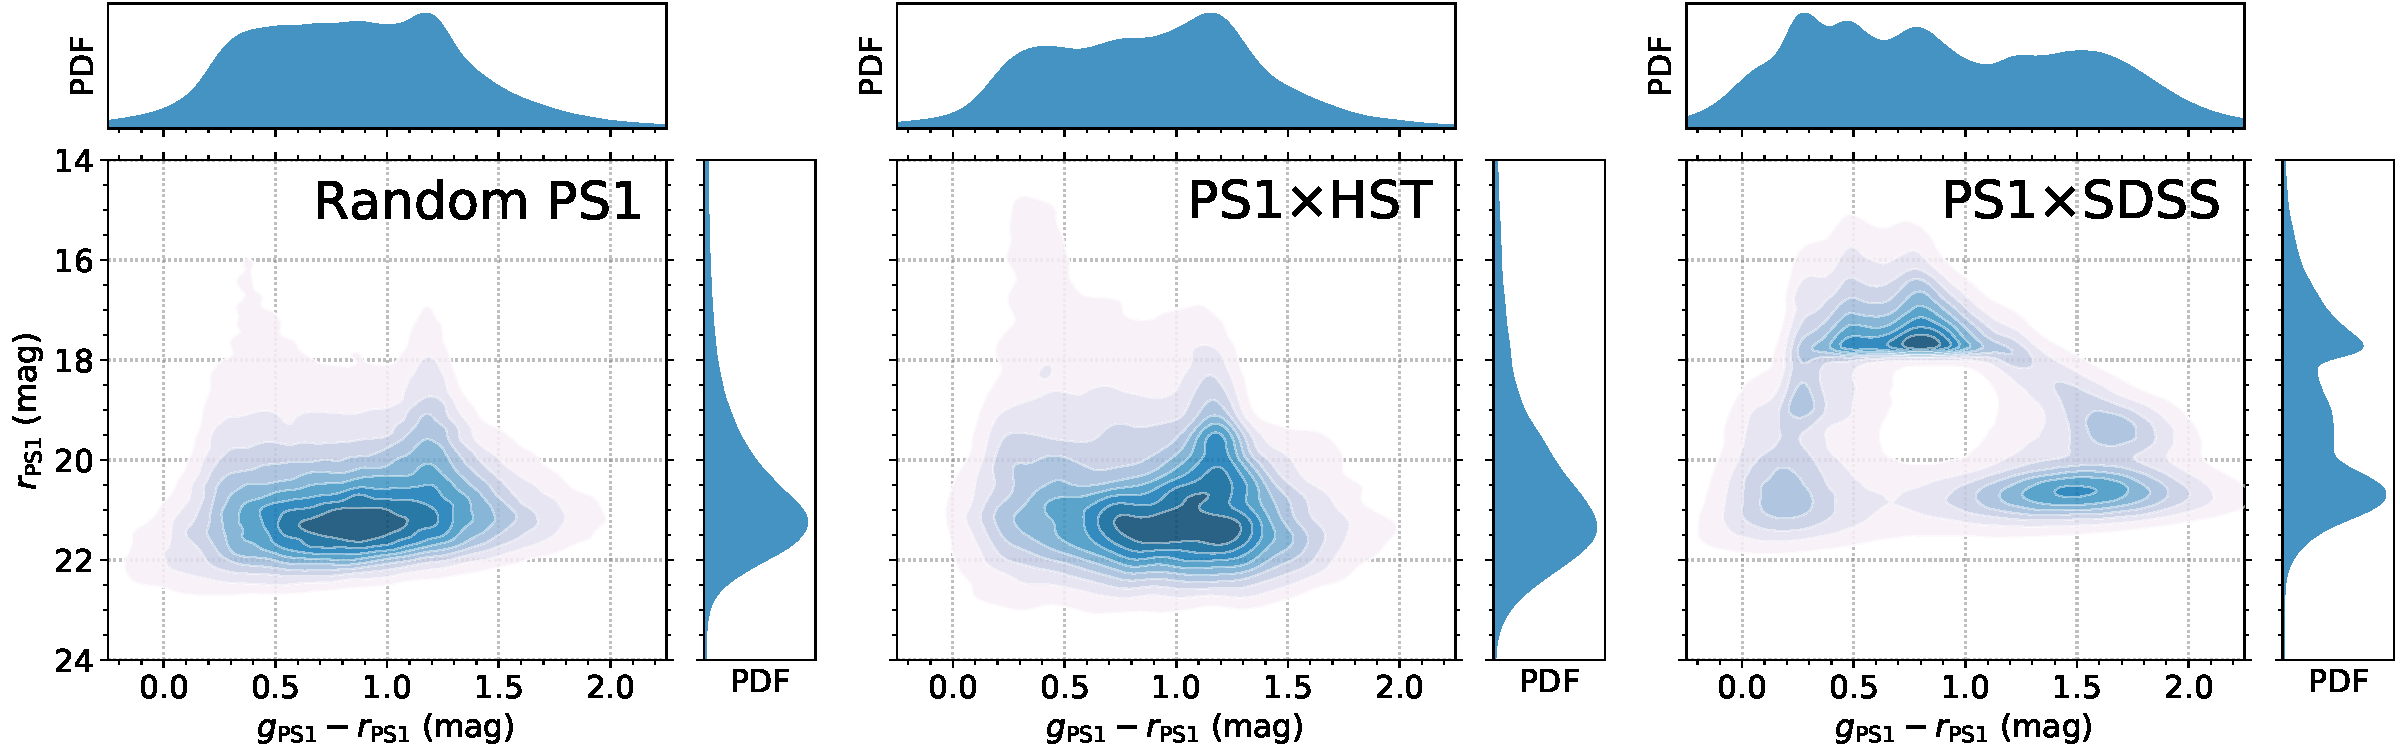
\includegraphics[width=7.2in]{./Figures/ColorMagDiagram.pdf}
  %
  \caption{ PS1 color-magnitude diagrams for \textit{left}: $10^6$ randomly
  selected sources, \textit{center}: the \textit{HST} training set, and
  \textit{right}: the SDSS training set. The primary panels show a
  two-dimensional (2D) Gaussian kernel density estimate (KDE) of the
  probability density function (PDF) of each subset of sources in the
  $r_\mathrm{PS1}$--$g_\mathrm{PS1} - r_\mathrm{PS1}$ plane. The shown
  contour levels extend from 0.9 to 0.1 in 0.1 intervals. To the top and
  right of the primary panels are marginalized 1D KDEs of the PDF for the
  $g_\mathrm{PS1} - r_\mathrm{PS1}$ color and $r_\mathrm{PS1}$ brightness,
  respectively. Kron aperture measurements from the \textit{StackObjectThin}
  table are used to estimate each of the PDFs. }
  %
  \label{fig:cmd}
\end{figure*}

The SDSS spectroscopic catalog classifies everything it observes as either a
star, galaxy, or quasi-stellar object (QSO). Using a $1\arcsec$ cross-match
radius, we find 3,834,627 sources with SDSS optical spectra have PS1
counterparts (hereafter, the SDSS training set). Thus, with an orders of
magnitude larger training set, and spectroscopic classifications that should
be pristine and superior to mophological clsasifications, one might expect
the SDSS training set to be optimal for training the machine learning model.
However, as noted in \citep{Miller17}, the SDSS spectroscopic targeting
algorithms were highly biased, and as a result prove challenging as a
training set.

Color-magnitude diagrams (CMDs) of the \textit{HST} and SDSS training sets
are compared to a random selection of $10^6$ sources from the PS1 database in
Figure~\ref{fig:cmd}. It is clear from Figure~\ref{fig:cmd} that the SDSS
training set is completely different from typical sources in PS1 and that
there are few SDSS sources in the highest density regions of the PS1 CMD.
Given the stark mismatch between typical PS1 sources and the SDSS training
set, we adopt the \textit{HST} training set for the development of our model.
We retain the SDSS training set as an independent test set to assess the
accuracy of the model following construction.

\section{Model Features}\label{sec:model_features}

In addition to developing a training set, we must select features to use as an input for the model. As noted in \S\ref{sec:model_data}, the PS1 database provides flux and shape measurements in each of the $grizy_\mathrm{PS1}$ filters. Adopting each of these measurements as features for the model presents a significant problem: missing data. There are relatively few sources in the PS1 database that are detected in all 5 filters. Typically, to cope with missing data one can either (i) remove sources detected in fewer than 5 filters, or (ii) assign some value, via either imputation (e.g., \citealt{Miller17}) or the use of a dummy variable, to the missing data. Given that the vast majority of PS1 sources are faint and are not detected in all 5 filters, neither of these possiblities is attractive for our present purposes.

Rather than use the raw features from the database, we engineer a series of ``white flux'' features that combine the relevant measurements across all filters in which a source is detected. In a given filter, a source is detected if the $\mathtt{PSFFlux}_f$, $\mathtt{KronFlux}_f$, and $\mathtt{ApFlux}_f$ are \textit{all $> 0$}, where the $f$ subscript refers to a specific filter. The ``white flux'' feature is then created as:
%
\begin{equation}
    \mathtt{white[Feat]} =  \frac{\sum_f^{f = grizy_\mathrm{PS1}} w_f  \, \mathtt{Feat}_f \, \mathrm{det}_f}{\sum_f^{f = grizy_\mathrm{PS1}} w_f}, 
\end{equation}
%
where the sum is over the 5 PS1 filters, \texttt{Feat} is the feature from the \textit{StackObjectAttributes} table, $\mathrm{det}_f = 1$ if the source is detected in the $f$ filter, as defined above, or $\mathrm{det}_f = 0$ if not detected, and $w_f$ is the weight assigned to each filter:
%
\begin{equation}
    w_f = \left(\frac{\mathtt{KronFlux}_f}{\mathtt{KronFluxErr}_f}\right)^2,
\end{equation}
%
equivalent to signal-to-noise ratio (SNR) squared in the given filter. Ultimately, the ``white flux'' features correspond to a weighted mean, with weights equal to the square of the SNR. 

Our final model includes 11 ``white flux'' features to separate stars and
galaxies. The database features include: \texttt{PSFFlux},\footnote{For the
\texttt{PSFFlux} feature $w_f =
(\mathtt{PSFFlux}_f/\mathtt{PSFFluxErr}_f)^2$.} \texttt{KronFlux},
\texttt{ApFlux},\footnote{For the \texttt{ApFlux} feature $w_f =
(\mathtt{PSFFlux}_f/\mathtt{PSFFluxErr}_f)^2$.}. 
\texttt{ExtNSigma},
\texttt{KronRad}, \texttt{psfChiSq}, \texttt{psfLikelihood},
\texttt{momentYY}, \texttt{momentXY}, \texttt{momentXX}, and
\texttt{momentRH}.\footnote{Prior to their ``white flux'' calculation the
shape features (\texttt{KronRad}, \texttt{momentYY}, \texttt{momentXY},
\texttt{momentXX}, and \texttt{momentRH}) are normalized by the seeing in the
respective bandpass, which we define as the \texttt{psfMajorFWHM} and
\texttt{psfMinorFWHM} added in quadrature. \texttt{KronRad} has units of
arcsec, \texttt{momentRH} has units of arcsec$^{0.5}$, and the remaining
shape features have units of arcsec$^{2}$. They are each normalized by
dividing by the seeing raised to the appropriate power. } The remaining
features in the database were either uninformative or would bias the model,
such as R.A.\ and Dec.\ (see e.g., \citealt{Richards12a}). We do not directly
include \texttt{whitePSFFlux}, \texttt{whiteKronFlux}, and
\texttt{whiteApFlux} in the model. We found that the inclusion of these
features resulted in a bias whereby all sources brighter than $\sim$16\,mag
were automatically classified as stars. Instead, we include the ratio of the
different flux measures: \texttt{whitePSFKronRatio} =
\texttt{whitePSFFlux}/\texttt{whiteKronFlux}, \texttt{whitePSFApRatio} =
\texttt{whitePSFFlux}/\texttt{whiteApFlux}, as well as a third feature
\texttt{whitePSFKronDist} (see \S\ref{sec:simple_model}).

As we previously alluded to, the primary benefit of the ``white flux''
features is that they can be calculated for every source in PS1 thus allowing
each to be compared on common ground. Furthermore, the SNR for the ``white
flux'' features is greater than the SNR for the equivalent feature in a
single filter. The downside of these features is that for some sources,
especially at the bright end, color information is lost. While a blue source
and red source with identical \texttt{whitePSFFlux} values are intrinsically
very different, the ``white flux'' features obscure that information for the
classifier. Ultimately, we tested models with and without the ``white flux''
features and found that they are statistically equivalent when tested with
the \textit{HST} training set.

The direct use of color information as model features would require reddening
corrections for all PS1 sources. Not only is this a daunting task, but
accurate corrections would require a priori knowledge as to which sources are
Galactic and which are extragalactic (e.g., \citealt{Green15}). The PS1
catalog is being developed precisely to answer this question. Furthermore,
the pencil beam sample from the \textit{HST} training set traces a narrow
range of dust columns, so the application of a model including color
information without reddening corrections would lead to biased
classifications 
\NC{
\citep{Sevilla18},}
 particularly in regions of high reddening (e.g., the
Galactic plane). We conclude that the benefits of the ``white flux''
features, which eliminate the need for reddening corrections, outweigh any
losses from the exclusion of color information.

\begin{figure*}[htb]
 \centering
  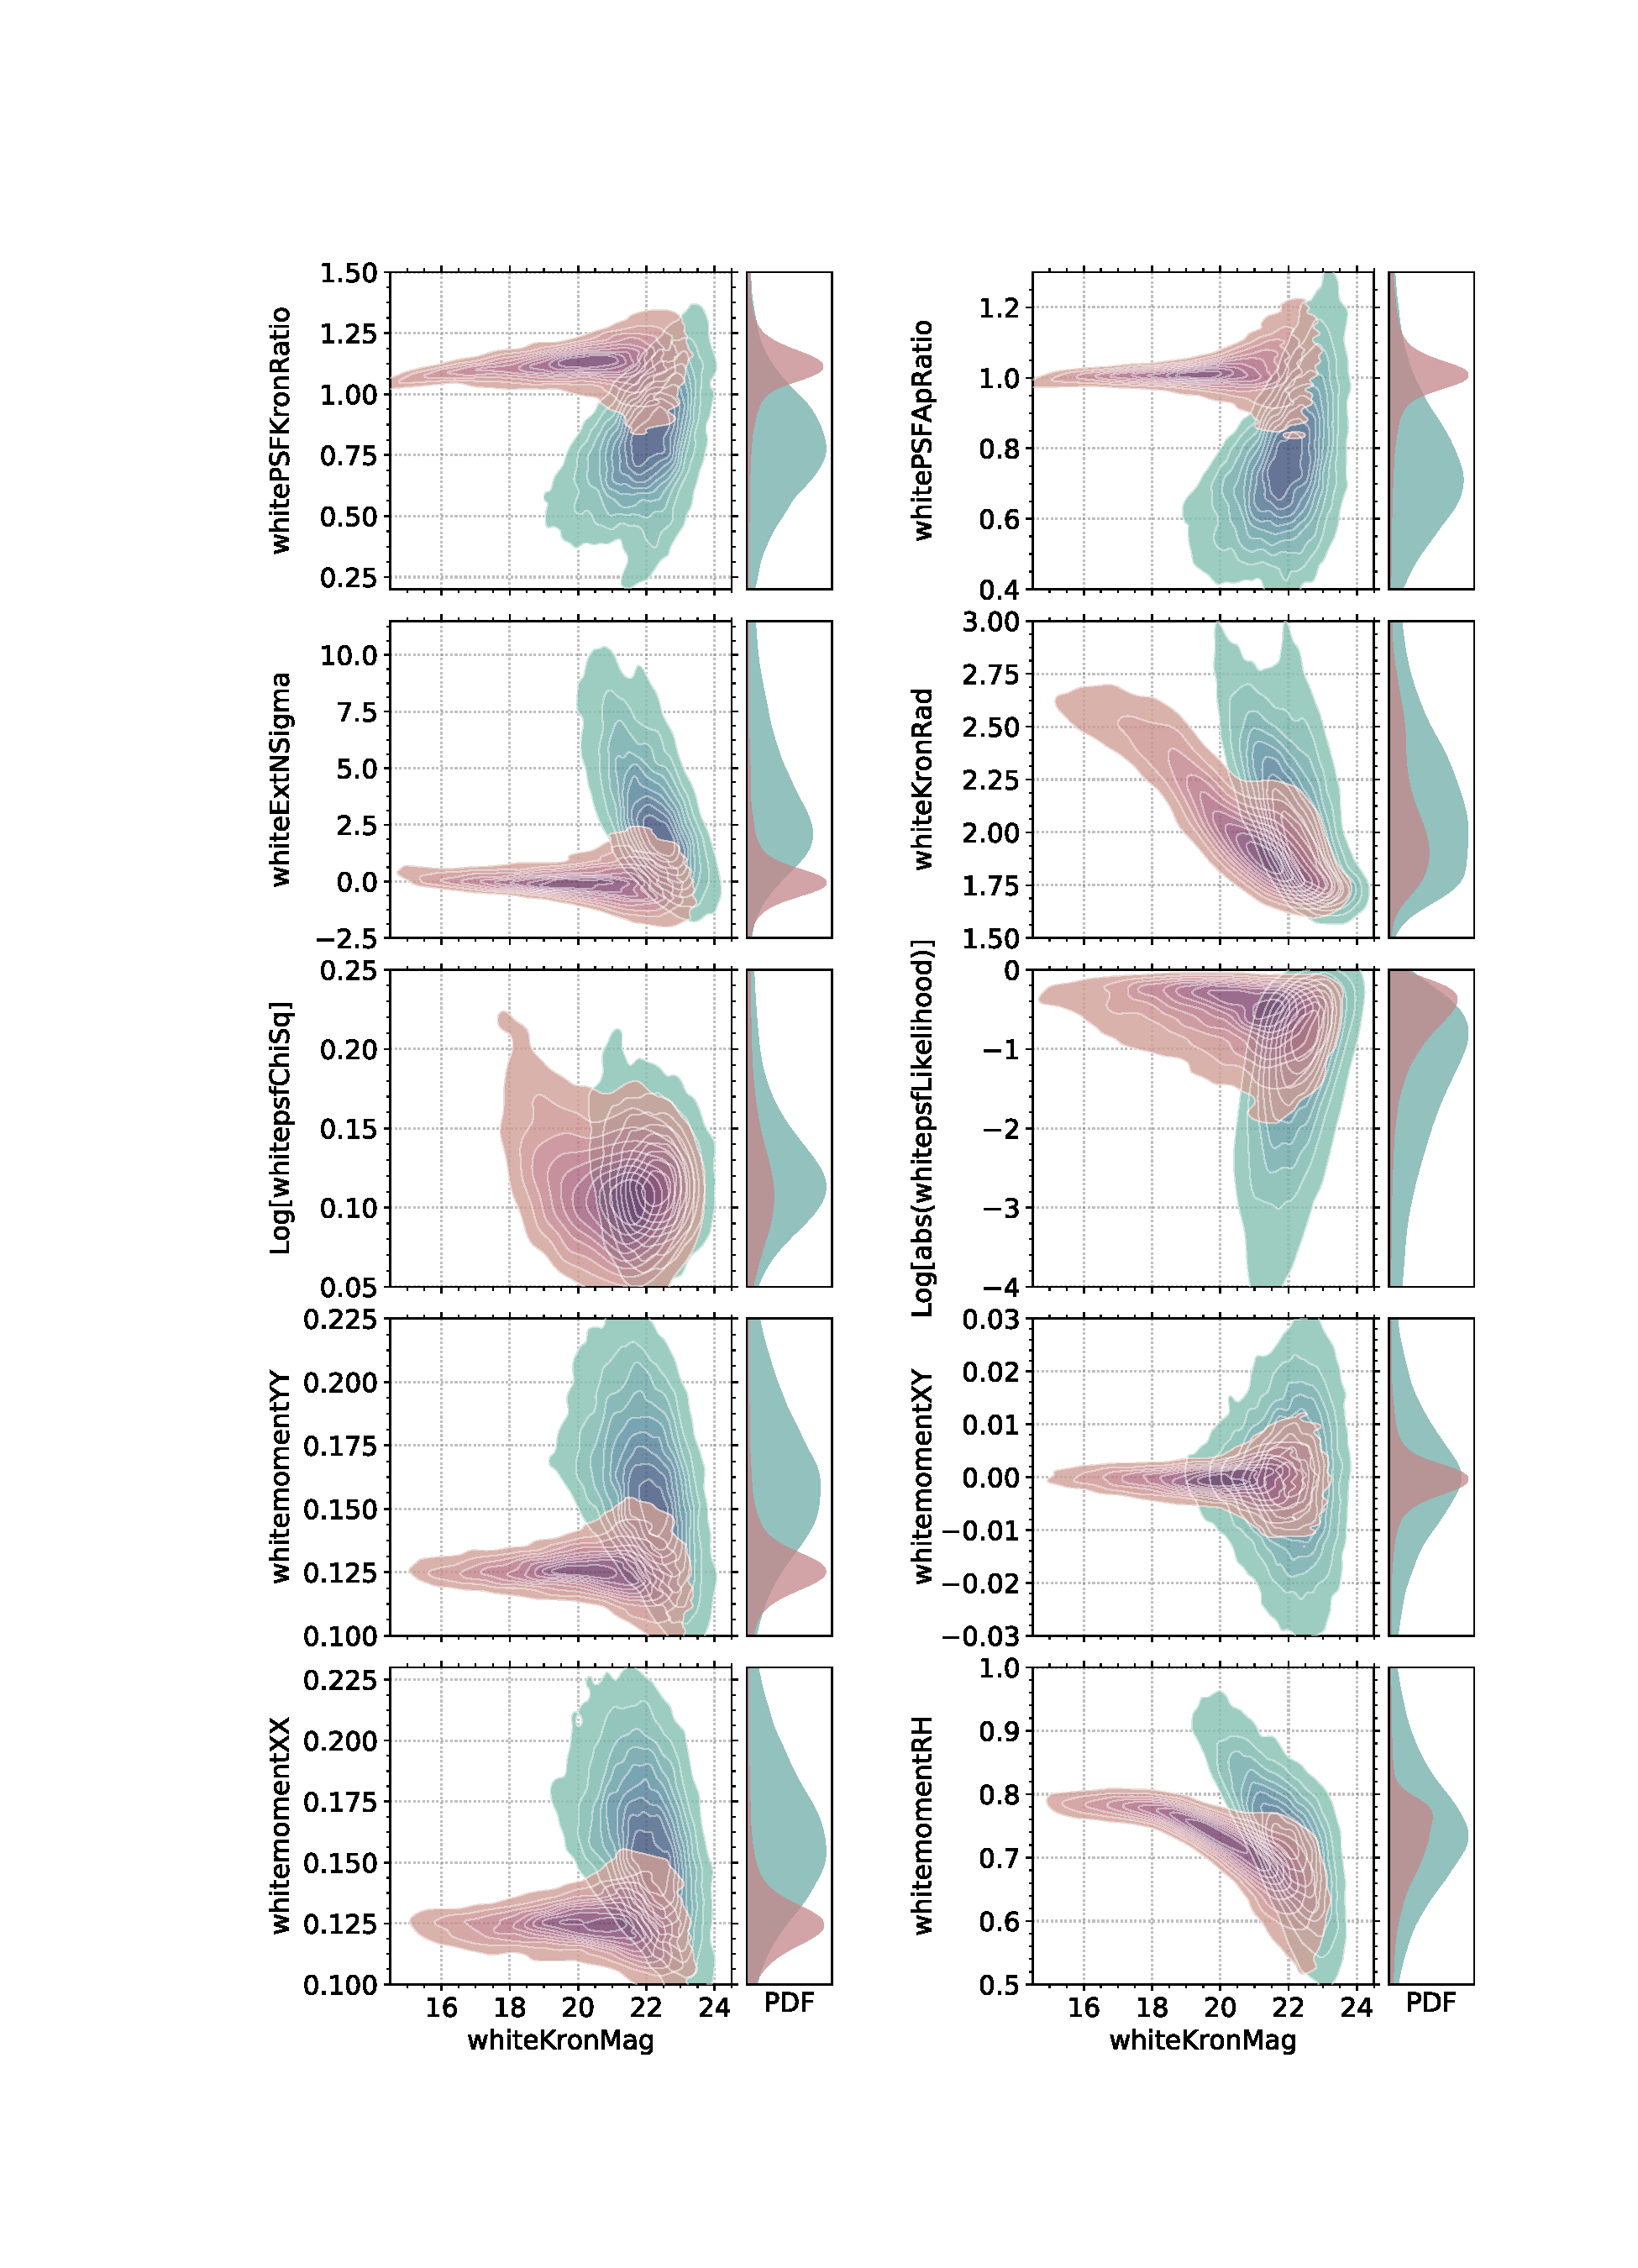
\includegraphics[width=5.75in]{./Figures/whiteFeatures.pdf}
  \caption{
  The primary square panels show KDEs of the PDF for each of the ``white
  flux'' features as a function of \texttt{whiteKronMag}
  ($=-2.5\log_{10}[\mathtt{whiteKronFlux}/3631]$) for all sources in the
  \textit{HST} training set. Stars are shown via the red-purple contours,
  while galaxies are shown via blue-green contours. The shown contour levels
  extend from 0.9 to 0.1 in 0.1 intervals. To the right of each primary panel
  is a marginalized 1D KDE of the PDF for the individual features, where the
  amplitudes of the KDEs have been normalized by the relative number of stars
  and galaxies. The clear overlap between faint stars and galaxies suggests
  that a machine learning model may provide significant improvement over the
  PS1 and simple models.}
  %
  \label{fig:features}
\end{figure*}

The distribution of ``white flux'' features for stars and galaxies in the
\textit{HST} training set is shown in Figure~\ref{fig:features}
(\texttt{whitePSFKronDist} is shown in Figure~\ref{fig:psfkrondist}). As
might be expected, it is clear from Figure~\ref{fig:features} that stars and
galaxies are easily separated at the bright end ($\lesssim 20$\,mag), but
there is significant overlap in the featurespace between the two populations
at the faint end ($\sim$23\,mag). Machine learning algorithms are capable of
capturing non-linear behavior in multidimentional data sets, which will
prove especially useful for the sources under consideration in the PS1 data
set.

\section{Model Construction}
\subsection{The PS1 Baseline Model}\label{sec:ps1_model}

To establish a baseline for the performance of our star-galaxy separation
models we adopt the classification criteria in the PS1 documentation, namely
sources with 
%
$$ \mathtt{iPSFMag} - \mathtt{iKronMag} > 0.05\;\mathrm{mag},$$
%
are classified as
galaxies.\footnote{\url{https://outerspace.stsci.edu/display/PANSTARRS/How+to+
separate+stars+and+galaxies}} The documentation notes that this
classification can be performed using photometry from any of the
\textit{MeanObject}, \textit{ForcedMeanObject}, or \textit{StackedObjectThin}
tables. The PS1 documentation further notes that this basic cut does not
perform well for sources with $i \gtrsim 21\,\mathrm{mag}$, which constitutes
the majority of sources detected by PS1, and motivates us to develop
alternative models. We use the performance of the $\mathtt{iPSFMag} -
\mathtt{iKronMag} > 0.05\;\mathrm{mag}$ model (hereafter, the PS1 model) as a
baseline to compare to the models discussed below.

\subsection{Simple Model}\label{sec:simple_model}

While our ultimate goal is to build a machine learning model to separate
stars and galaxies (\S\ref{sec:rf_model}), we first construct a
straightforward model. This model is inspired by the SDSS \texttt{photo}
pipeline \citep{Lupton01}, and combines the flux in each of the 5 PS1 filters
to improve the SNR relative to any individual band. In addition to being easy
to interpret, this model (hereafter, the simple model), which utilizes the
difference between the PSF flux and the Kron-aperture flux for
classification, serves as an additional baseline to test the need for a more
complicated machine learning model.

It stands to reason that a model built on all five PS1 filters should outperform a model constructed from a single filter. To that end, we examine the \texttt{whitePSFKronRatio} (equivalent to $\mathtt{whitePSFMag} - \mathtt{whiteKronMag}$) to discriminate between stars and galaxies. The upper left panel of Figure~\ref{fig:features} shows that sources with $\mathtt{whitePSFKronRatio} \gtrsim 1$ are very likely to be stars. A single hard cut on \texttt{whitePSFKronRatio}, similar to the SDSS \texttt{photo} pipeline or the PS1 model, removes any sense of confidence in the corresponding classification. For example, a source with $\mathtt{whitePSFKronRatio} = 1.1$ and $\mathtt{whiteKronMag} \approx 17\,\mathrm{mag}$ is far more likely to be a star than a source with the same \texttt{whitePSFKronRatio} value but $\mathtt{whiteKronMag} \approx 23\,\mathrm{mag}$ (see Figure~\ref{fig:features}).

To address this issue of classification confidence, we measure the
orthogonal distance from a line ($\mathtt{whitePSFFlux} = a\times
\mathtt{whiteKronFlux}$) for all sources in the
$\mathtt{whitePSFFlux}$--$\mathtt{whiteKronFlux}$ plane to define the simple model:
%
\begin{multline}
 \mathtt{whitePSFKronDist}(a) = \\
 \frac{\mathtt{whitePSFFlux} - a\times\mathtt{whiteKronFlux}}{ \sqrt{1 + a^2}},
 \label{eqn:psfkrondist}
\end{multline}
%
where $a$ is the slope of the line. For $a \approx 1$, which is similar to a
hard cut with $\mathtt{whitePSFKronRatio} = a$, bright stars will have
large, positive values of \texttt{whitePSFKronDist}, while bright galaxies
will have large, negative values of \texttt{whitePSFKronDist}.
Simultaneously, faint sources, which are more difficult to classify, will
have small values of \texttt{whitePSFKronDist}. The simple model allows us
to produce a rank ordered classification, which in turn allows us to
evaluate the optimal classification threshold for the separation of stars
and galaxies (see \S\ref{sec:comp_hst}).

The optimal value for $a$ is determined via $k$-fold cross validation (CV).
We adopt identical procedures to optimize both the simple model and the
machine learning model (see \S\ref{sec:rf_model}). We employ the use of an
inner and outter CV loop, both of which have $k = 10$ folds. In the outter
CV loop, the training set is split into 10 separate partitions, each
iteratively withheld from the training. For each partition in the outter CV
loop, an inner 10-fold CV is applied to the remaining $\sim$90\% of the
training set to determine the optimal model parameters. Predictions on the
sources withheld in the outter loop are made with the optimal model from the
inner loop to provide model predictions for every source in the training
set. We adopt final, optimal tuning parameters from the mean of the values
determined in the inner CV.

For the simple model, we employ a grid search over $a$ in the inner CV loops
to maximize the FoM and thereby determine the optimal value of $a$.
Initially, a wide grid from 0 to 2 was searched, followed by a fine grid
search over $a$ from 0.75 to 1.25 with step size = 0.0025. The average
optimal $a$ from the inner loops, and hence final model value, is 0.91375,
with sample standard deviation $\sim$0.01. From this procedure, we find that
for the simple model the $\mathrm{FoM} = 0.62 \pm 0.02$, where the
uncertainty is estimated from the scatter in the outter CV
results.\footnote{We find that PS1 flux measurements from the
\textit{StackObjectThin} table produce a higher FoM for the simple model
than flux measurements from the \textit{MeanObject} and
\textit{ForcedMeanObject} tables. Thus, we adopt \textit{StackObjectThin}
fluxes for both the simple model and the machine learning model, as noted in
\S\ref{sec:model_data}.}


\begin{figure}[t]
 \centering
  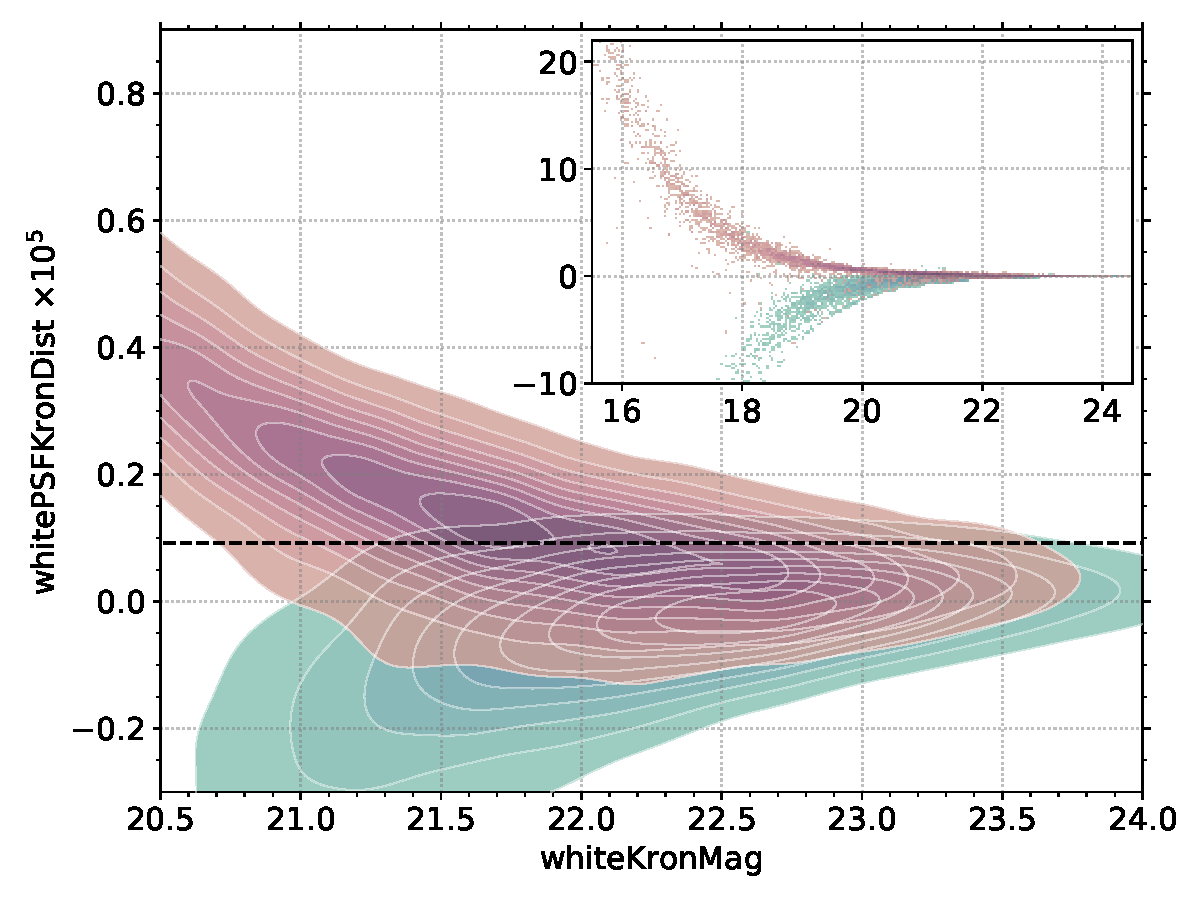
\includegraphics[width=3.35in]{./Figures/whitePSFKronDist.pdf}
  %
  \caption{ The distribution of $\mathtt{whitePSFKronDist}$ values for
  \textit{HST} training set stars and galaxies as a function of
  \texttt{whiteKronMag}. The colors and contours are the same as
  Figure~\ref{fig:features}. The horizontal dashed line shows the optimal
  threshold ($\mathtt{whitePSFKronDist} \ge 9.2 \times 10^{-7}$) for
  star--galaxy classification. The upper-right inset shows a zoom-out
  highlighting the stark difference between stars and galaxies at the bright
  end. }
  %
  \label{fig:psfkrondist}
\end{figure}

The distribution of $\mathtt{whitePSFKronDist}(a=0.91375)$ is shown for
\textit{HST} training set stars and galaxies in
Figure~\ref{fig:psfkrondist}. $\mathtt{whitePSFKronDist}$ provides an
excellent discriminant between bright ($\lesssim 20\,\mathrm{mag}$) stars
and galaxies. We further find that adopting a stellar classification
threshold of $\mathtt{whitePSFKronDist} \ge 9.2 \times 10^{-7}$ produces a
classification accuracy of $\sim$91\%.

\subsection{Random Forest Model}\label{sec:rf_model}

\subsubsection{The Random Forest Algorithm}\label{sec:rf_alg}

Based on its success in previous astronomical applications (e.g., \citealt{Richards12a, Huppenkothen17, Brink13, Wright15, Goldstein15}), including
star--galaxy separation (e.g., \citealt{Vasconcellos11,Miller17}), we adopt
the RF algorithm \citep{Breiman01} for our machine learning model. Briefly,
RF is built on decision tree models \citep{Quinlan93} that utilize bagging
\citep{Breiman96}, wherein bootstrap samples of the training set are used to
train each of the $N_{\mathrm{tree}}$ individual trees. Within the
individual trees, only $m_{\mathrm{try}}$ randomly selected features are
used to separate sources at each node, and nodes cannot be further split if
there are fewer than \texttt{nodesize} sources in the node. The randomness
introduced by both bagging and the use of $m_{\mathrm{try}}$ features
reduces the variance of RF predicitions relative to single decision tree
models. Final RF classifications are determined via a majority vote from
each of the $N_{\mathrm{tree}}$ individual trees. Thus, RF models are
capable of producing low-variance, low-bias predictions. We utilize the
\texttt{Python scikit-learn} implementation of the RF algorithm
\citep{Pedregosa12} in this study.

\subsubsection{Feature Selection}

While the RF algorithm is relatively insensitive to correlated and/or
weak/uninformative features (e.g., \citealt{Richards12a}), we nevertheless
investigate if removing features from our feature set improves the model
performance.\footnote{For example, we find a strong correlation between
\texttt{whiteExtNSigma} and \texttt{whitepsfLikelihood} (Pearson correlation
coefficient $r = 0.85$), which can potentially lead to overfitting.} We do
this via forward and backward feature selection \citep{Guyon03}. Forward and
backward feature selection involve the iterative addition or removal of
features from the model, respectively. Like \citet{Richards12a}, we rank
order the features for either addition or subtraction based on their
RF-determined importance \citep{Breiman02}. In either case, we find that
removing features does not improve the CV FoM, and therefore include all 11
features from \S\ref{sec:model_features} the final RF model.

\subsubsection{Optimizing the Model Tuning Parameters}

As noted in \S\ref{sec:simple_model}, we optimize the RF model tuning
parameters via an outter and inner 10-fold CV procedure. We perform a grid
search over $N_{\mathrm{tree}}$, $m_{\mathrm{try}}$ and \texttt{nodesize},
and find that the FoM of \textit{HST} training is maximized with
$N_{\mathrm{tree}} = 400$, $m_{\mathrm{try}} = 4$, and $\mathtt{nodesize} =
2$. The final model FoM is not strongly sensitive to the choice of these
parameters: changing any of the optimal parameters by a factor of $\sim$2
does not decrease the optimal CV FoM, 0.71, by more than the scatter
measured from the individual folds, 0.02. Finally, while a detailed
comparison is presented in \S\ref{sec:comp_hst}, we note that the RF model
significantly outperforms the simple model based on the CV FoM.

\section{Classification Performance}

\subsection{PS1, Simple, and RF Model Comparison}\label{sec:comp_hst}

We assess the relative performance of the RF model by comparing it to both
the PS1 and simple models. To do so, we select the subset of sources from
the \textit{HST} training set that have $\mathrm{det}_{i_\mathrm{PS1}} = 1$
(the PS1 model cannot classify sources that are not detected in the
$i_\mathrm{PS1}$ band), which results in 40,098 sources.

Figure~\ref{fig:cvroc_hst} shows that the RF model and simple model provide
substantial improvements over the PS1 model, with $\sim$10,000\% and
$\sim$9,200\% respective increases in the FoM relative to the PS1 model. We
additionally show Receiver Operating Characteristic (ROC) curves for the 3
models in Figure~\ref{fig:cvroc_hst}. ROC curves show how the true positive
rate (TPR)\footnote{$\mathrm{TPR} = \mathrm{TP}/(\mathrm{TP} +
\mathrm{FP})$, where TP is the total number of true positive classifications
and FP is the number of false positives.} and false positive rate
(FPR)\footnote{$\mathrm{FPR} = \mathrm{FP}/(\mathrm{FP} + \mathrm{TN})$,
where TN is the number of true negatives.} vary as a function of
classification threshold. As a reminder, stars are considered the positive
class in this study. To construct ROC curves for the simple and PS1 models
we vary the classification thresholds from $\mathrm{whitePSFKronDist} =
4.24\times 10^{-3}$ to $-16.23\times10^{-3}$ and $\mathtt{iPSFMag} -
\mathtt{iKronMag} = 5.10\;\mathrm{mag}$ to $-2.81\;\mathrm{mag}$,
respectively. Figure~\ref{fig:cvroc_hst} highlights the strength of the
simple model approach: by using a metric that essentially captures both the
difference between the PSF and Kron-aperture measurements \textit{and} the
SNR, the simple model produces much higher TPR at low FPR than the PS1
model, which eliminates any information about the SNR.

Summary statistics showing the superior performance of the RF model relative
to the simple and PS1 models are presented in Table~\ref{tbl:hst_cv}.
These statistics include the FoM, the integrated area under the ROC curve
(ROC AUC), and the overall accuracy of the 3 models as evaluted on the
subset of \textit{HST} training set sources with $i_\mathrm{PS1}$
detections. We use 10-fold CV to measure the summary statistics, with
identical folds for each model. Strictly speaking, this CV procedure is only
needed for the RF model, which needs to be re-trained for every fold, but
testing the simple and PS1 models on the individual folds provides an
estimate in the scatter of the final reported metrics. From
Table~\ref{tbl:hst_cv} it is clear that the RF model greatly outperforms
the simple and PS1 models.


\begin{deluxetable}{cccc}
    \tablecolumns{4} 
    \tablewidth{0pt} 
    \tablecaption{ CV Results for \textit{HST} Training Set \label{tbl:hst_cv}}
    \tablehead{ 
    \colhead{model} & \colhead{FoM} & \colhead{Accuracy} & \colhead{ROC AUC}
    }
    \startdata
    RF & {\bf 0.707} $\pm$ 0.036 & {\bf 0.932} $\pm$ 0.003 & {\bf 0.973} $\pm$ 0.002 \\
    simple & 0.657 $\pm$ 0.020 & 0.916 $\pm$ 0.003 & 0.937 $\pm$ 0.004 \\
    PS1 & 0.007 $\pm$ 0.003 & 0.810 $\pm$ 0.006 & 0.851 $\pm$ 0.006 \\
    \enddata
    \tablecomments{Uncertainties represent the sample standard deviation for the 10 individual folds used in CV.}
\end{deluxetable}

%%% fig:cvroc_hst %%%
\begin{figure}[t]
 \centering
  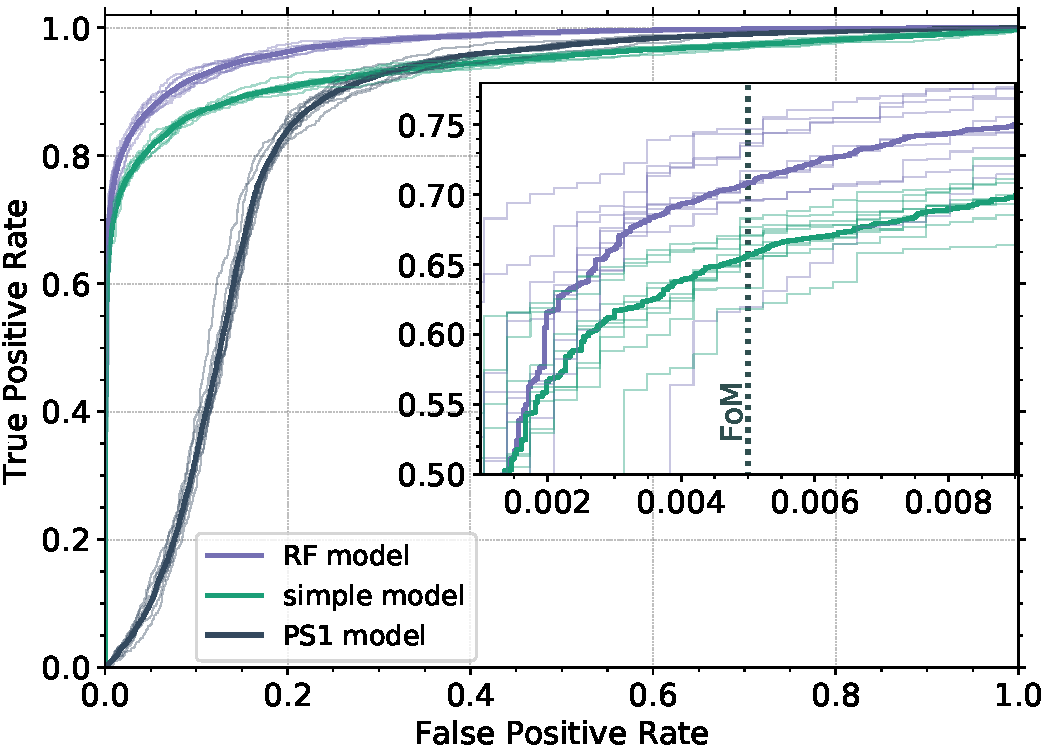
\includegraphics[width=3.35in]{./Figures/CV_ROC_HST.pdf}
  %
  \caption{ ROC curves comparing the relative performance of the PS1,
  simple, and RF models as tested by the subset of \textit{HST} training set
  sources with $i_\mathrm{PS1}$ detections. The thick, solid orange, blue,
  and black lines show the ROC curves for the PS1, simple, and RF models,
  respectively. The light, thin lines show the ROC curves for the individual
  CV folds. The inset on the right shows a zoom in around FPR = 0.005, shown
  as a dotted vertical line, corresponding to the FoM (the PS1 model is not
  shown in the inset, because it has very low FoM). }
  %
  \label{fig:cvroc_hst}
\end{figure}

\begin{figure}[t]
 \centering
  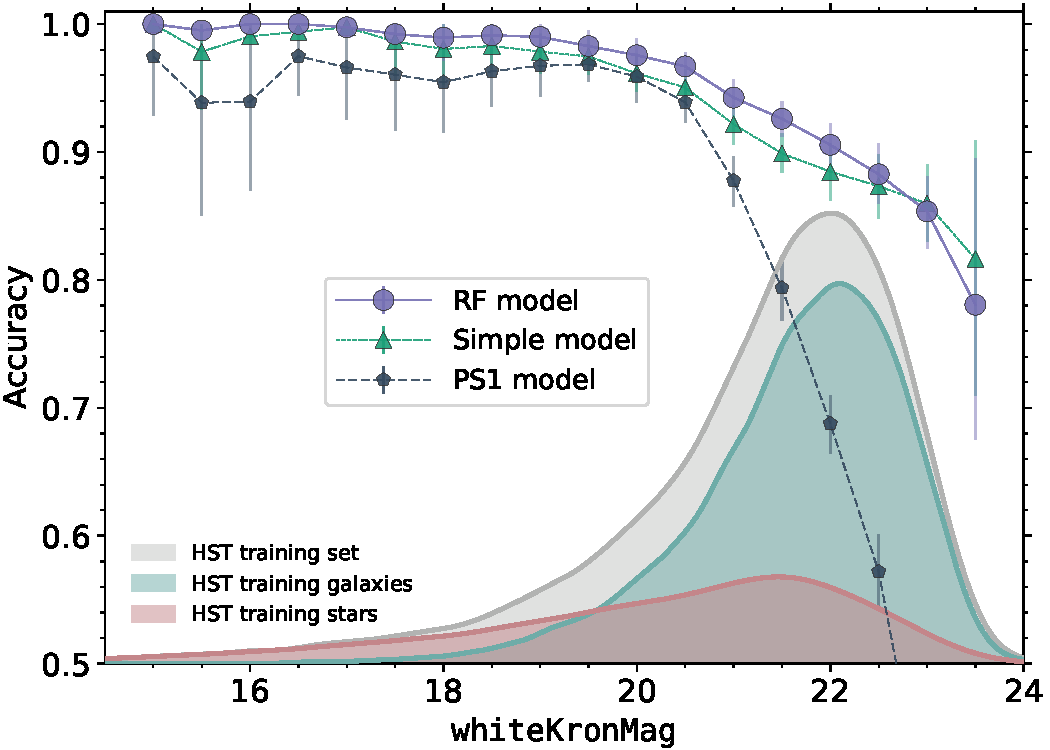
\includegraphics[width=3.35in]{./Figures/CV_Accuracy_HST.pdf}
  %
  \caption{Model accuracy as a function of \texttt{whiteKronMag} evaluated
  on the subset of the \textit{HST} training set sources with
  $i_\mathrm{PS1}$ detections. Accuracy curves for the PS1, simple and RF
  models are shown in orange, blue, and black, respectively. The bin widths
  are 0.5\,mag, and the error bars represent the 68\% interval from
  bootstrap resampling. Additionally, a Gaussian KDE of
  the PDF for the entire \textit{HST} training set subset, as well as the
  stars and galaxies in the subset is shown in the shaded grey, red, and
  green regions, respectively. The amplitude of the star and galaxy PDFs
  have been normalized by their relative ratio compared to the full subset. }
  %
  \label{fig:cvacc_hst}
\end{figure}
%%%%%%%%%%%%%

The classification accuracy for each model as a function of
\texttt{whiteKronMag} is shown in 0.5\,mag bins in
Figure~\ref{fig:cvacc_hst}. The accuracies are estimated via 10-fold CV (see
above) and the uncertainties represent the inter-68\% interval from
100 bootstrap samples within each bin. 
The classification thresholds for the RF, simple, and PS1 models are 0.5,
$9.2 \times 10^{-7}$, and 0.05, respectively. Again, the RF and simple
models provide a significant improvement over the PS1 model. The PS1 model
provides classification accuracies $\gtrsim$90\% for sources with
$\mathtt{whiteKronMag} \lesssim 21\,\mathrm{mag}$, but precipitously
declines for fainter sources. The RF and simple models have similar curves
with the RF model performing slightly better, as is to be expected given
that the RF model uses 10 additional features beyond
\texttt{whitePSFKronDist}.

\subsection{Model Evaluation via an Independent Test Set}

\begin{deluxetable}{cccc}
    \tablecolumns{4} 
    \tablewidth{0pt} 
    \tablecaption{SDSS Test Set Metrics\label{tbl:sdss_per}}
    \tablehead{ 
    \colhead{model} & \colhead{FoM} & \colhead{Accuracy\tablenotemark{a}} & \colhead{ROC AUC}
    }
    \startdata
    RF & \textbf{0.843} $\pm$ 0.001 & 0.9625 $\pm$ 0.0001 & \textbf{0.98713} $\pm$ 0.00007 \\
    simple & 0.798 $\pm$ 0.002  & 0.9557 $\pm$ 0.0001 & 0.98503 $\pm$ 0.00008 \\
    PS1 & 0.290 $\pm$ 0.004 & 0.9612 $\pm$ 0.0001 & 0.98411 $\pm$ 0.00007 \\
    SDSS & 0.777 $\pm$ 0.003 & \textbf{0.9713} $\pm$ 0.0001 & 0.98660 $\pm$ 0.00008 \\
    \enddata
    \tablecomments{Uncertainties represent the sample standard deviation for the 100 bootstrap resampling.} 
    \tablenotetext{a}{Classification accuracies are evaluated using classification cuts of $0.5$, $9.2 \times 10^{-7}$, $0.05$, and $0.145$ for the RF, simple, PS1, and SDSS models, respectively.}
\end{deluxetable}

%%% fig:roc_sdss %%%
\begin{figure}[t]
 \centering
  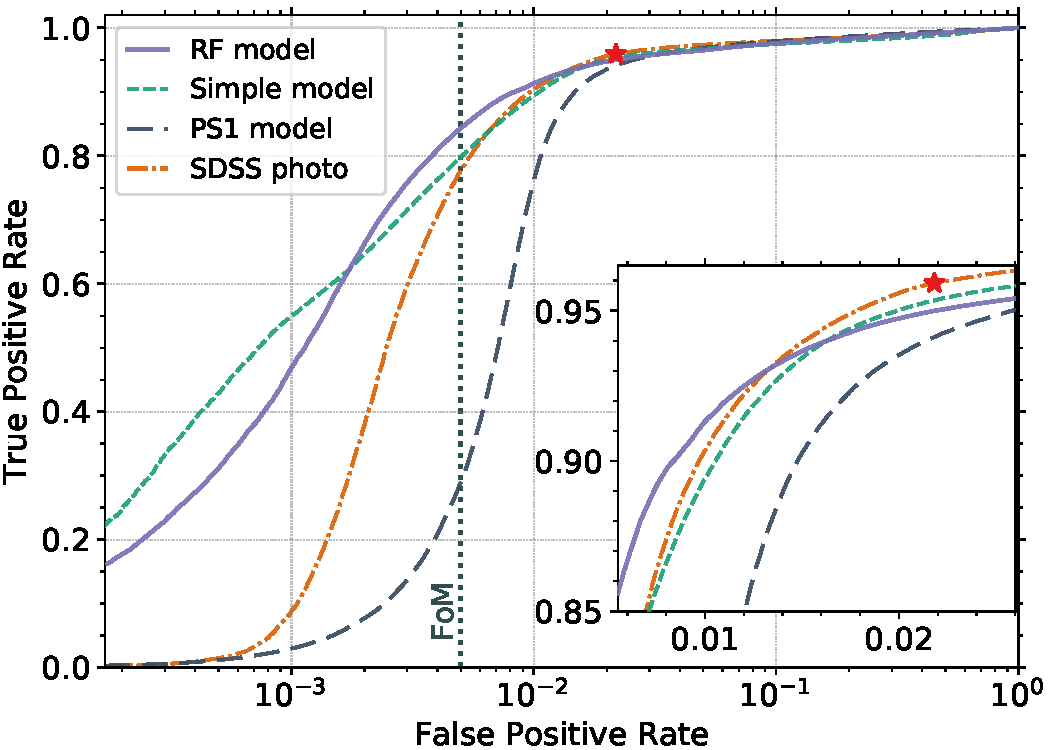
\includegraphics[width=3.35in]{./Figures/ROC_curves_log_inset2.pdf}
  %
  \caption{ ROC curves comparing the relative performance of the SDSS (orange
  dot-dashed line), PS1 (slate grey dashed line), simple (green dotted line),
  and RF (solid purple) models as tested by the SDSS test set. The vertical
  dotted line shows $\mathrm{FPR} = 0.005$, corresponding to the FoM. The
  inset shows a zoom in around the region where the ROC curves cross (see
  text for further details). The black and the red stars show the FPR and TPR
  if adopting the PS1 model and SDSS \textit{photo} classification cuts,
  respectively. The RF model delivers the highest FoM.}
  %
  \label{fig:roc_sdss}
\end{figure}
%%%%%%%%%%%%%

While CV on the \textit{HST} training set shows that the RF model
outperforms the alternatives, here, we test each of the previous models with
the SDSS training set, which provides an independent set of $\sim$3.8$\times
10^6$ sources with high-confidence
labels. Additionally, the use of SDSS spectra allows us to compare our new
models to the classifications from the SDSS \texttt{photo} pipeline,
hereafter the SDSS model, which soundly outperformed the PTF RF star--galaxy
model \citep{Miller17}. We create an ROC curve for the SDSS model by
thresholding on the ratio of PSF flux to \texttt{cmodel} flux measured in the
SDSS images (see \citealt{Miller17} for more details).

To compare the 4 models, we evaluate the performance of each model on the
subset of SDSS training set sources that have $i_\mathrm{PS1}$ detections
(to compare with the PS1 model) and SDSS \texttt{photo} classifications (to
compare with the SDSS model). We further exclude QSOs with $z < 1$ (=
133,856 sources; QSOs are typically considered point sources but low-$z$
QSOs can have resolved host galaxies; see \citealt{Miller17}), and galaxies
with $z < 10^{-4}$ (= 13,261 sources; such low $z$ is only expected in the
local group meaning most of these classifications are likely spurious). In
total, this subsample (hereafter the SDSS test set) includes 3,592,940
sources from the SDSS training set.

ROC curves for the RF, simple, PS1, and SDSS models, as measured by the SDSS
test set, are shown in Figure~\ref{fig:roc_sdss}. The FoM for the PS1,
simple, and RF models is higher as tested by SDSS spectroscopic sources
because the SDSS training set contains brighter, higher SNR (and hence
easier to classify) sources. As before, we find that the FoM for the RF
model is superior to the alternatives. Interestingly, we also find that the
ROC curves cross, and that the SDSS model provides the largest TPR for
$\mathrm{FPR} \gtrsim 0.015$. That the RF and SDSS curves cross suggests
that there may be regimes where the SDSS \texttt{photo} classifications are
superior to the RF model. Below, we argue that a bias in the SDSS training
set is amplified by a bias in the SDSS \texttt{photo} classification, which
is why these curves cross.

% Although the data set has the selection bias as mentioned above and thus the
% distribution of stars and galaxies as a function of brightness is totally
% different to that of the training set, the ROC curve of ML model is superior
% to the other models in terms of the FoM and also the ROC AUC; the FoM for
% the SDSS model, the PS1 model, the simple model, and the ML model is 0.777,
% 0.290, 0.798, and 0.843, respectively, and the ROC AUC score for each model
% is 0.987, 0.984, 0.985, and 0.987, respectively.

% Next, we assess the performance of the ML model by comparing with SDSS photometric classification
% by using PS1-SDSS spectroscopic catalog.
% Figure \ref{fig:roc_sdss} shows the ROC curve for
% the SDSS photo, the PS1 model, the simple model, and the ML model,
% by comparing predictions with SDSS spectroscopic classifications,
% which are independent of the training data set; PS1-HST cross-matched catalog.
% For sources in PS1-SDSS catalog, broadly,
% the performance of classifications by each model is better than that for sources in PS1-HST catalog.
% This is simply because that the distribution of sources, especially galaxies, in PS1-SDSS catalog
% are biased toward to brighter side comparing with of PS1-HST catalog.
% The selection bias of the SDSS spectroscopic survey
% toward observing luminous red galaxies (LRGs; {\it e.g.,} see \citealt{Eisenstein01})
% results in the KDE of the PDF of galaxies having two peaks
% at $\mathtt{whiteKronMag} \sim 17$ and $\sim 20$
% (see \S\ref{sec:sdss} and the left panel in Figure \ref{fig:acc_sdss}).
% As we alluded to in \S\ref{sec:comp_hst},
% the distribution of stars and galaxies in the real universe (except the galactic plane)
% should be similar to that shown in Figure \ref{fig:cvacc_hst};
% the peak of the distribution for stars and galaxies is around $\mathtt{whiteKronMag} \sim 22$
% and the number of stars and of galaxies is dominant at the bright end and the faint end,
% respectively \citep{Chambers16}.

%%% fig:acc_sdss %%%
\begin{figure*}[htb]
 \centering
  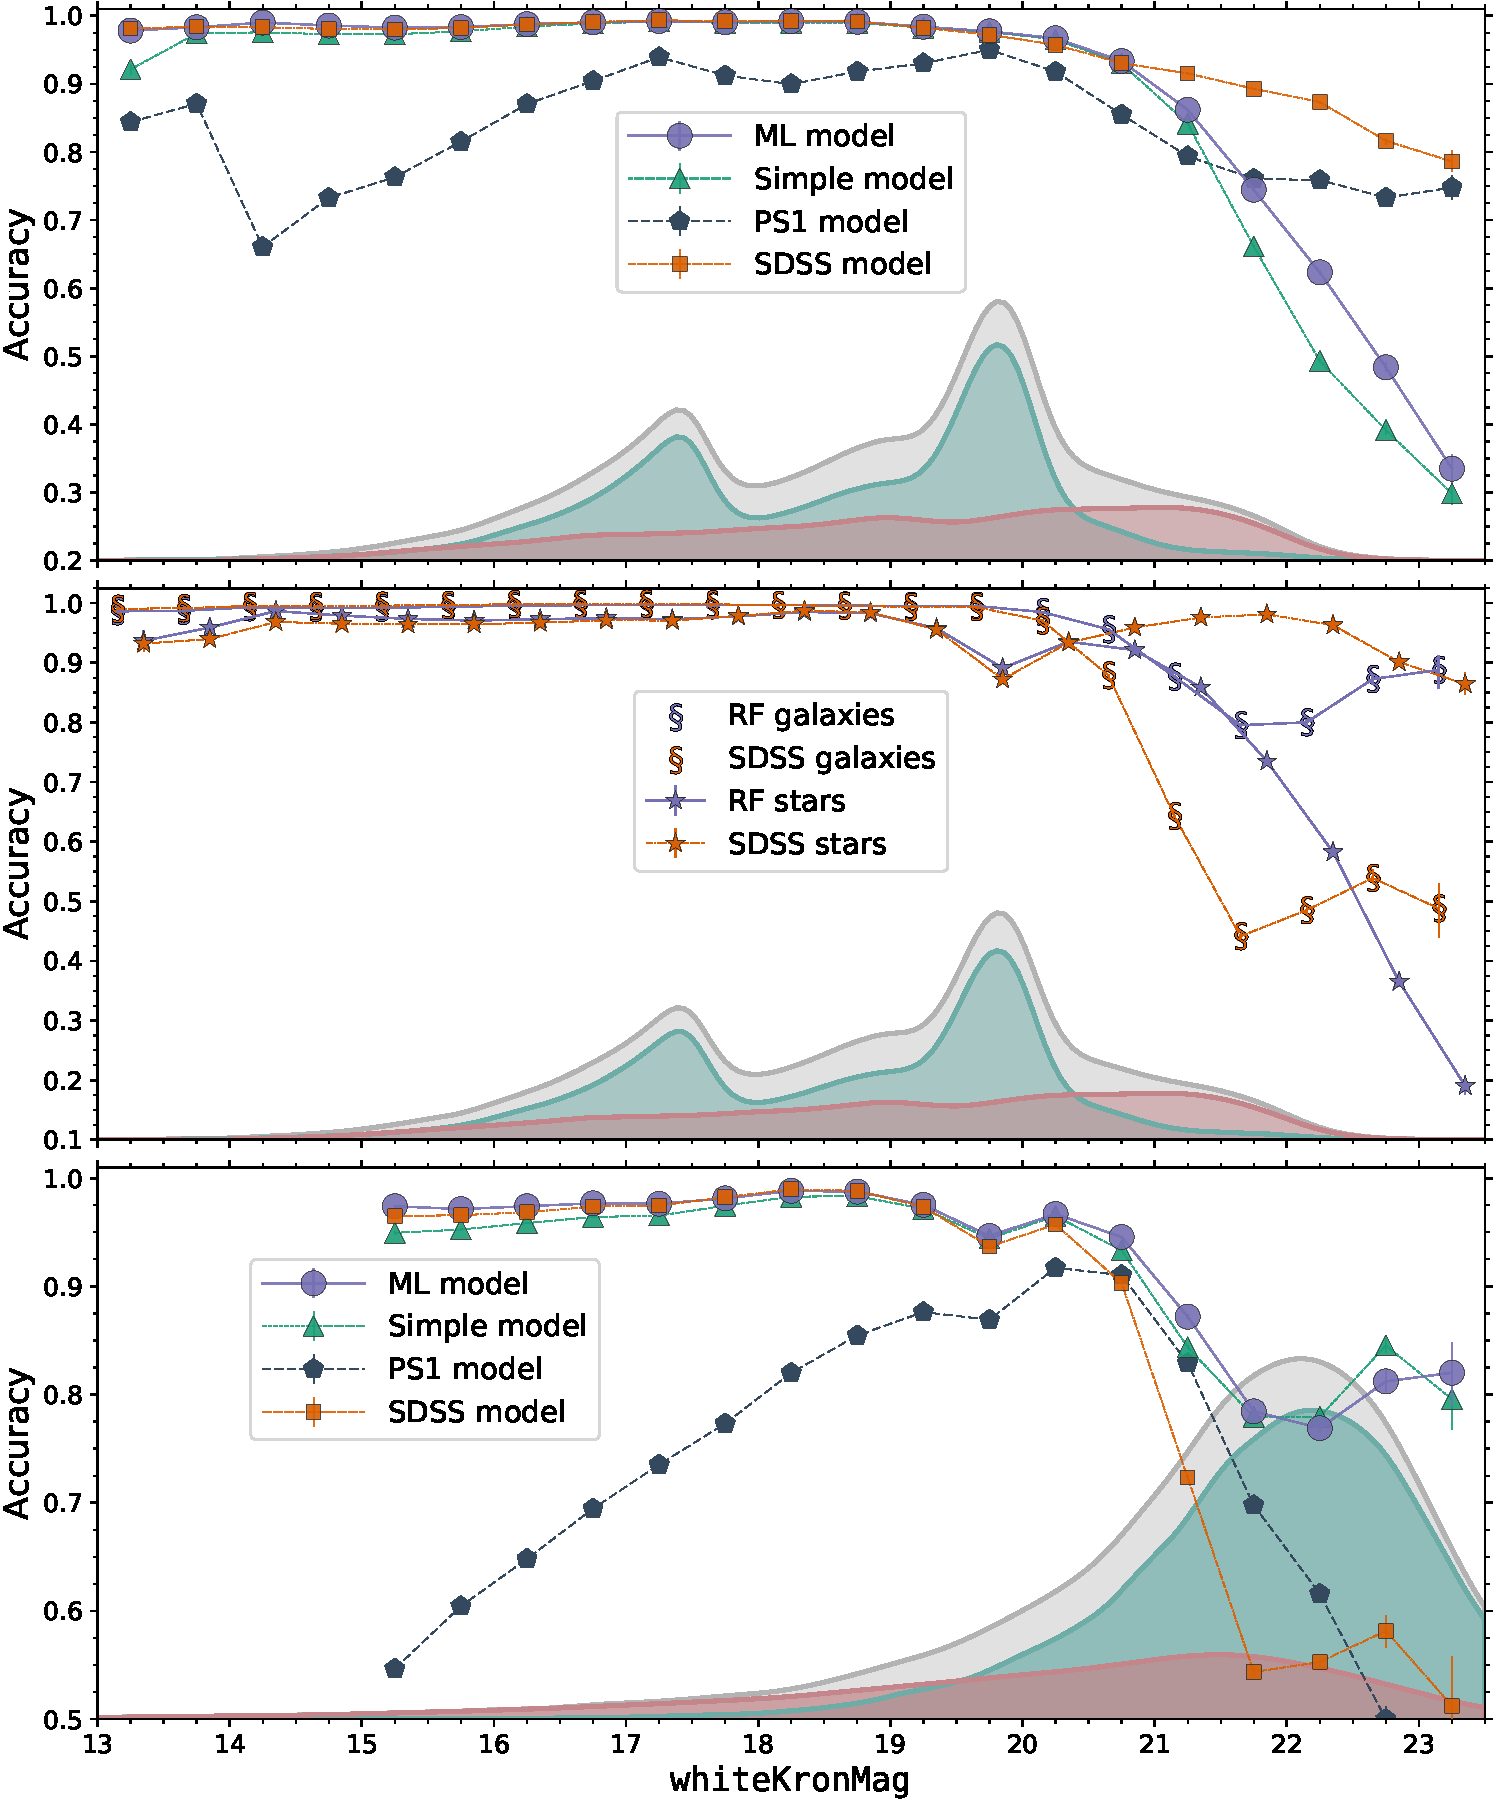
\includegraphics[width=6.2in]{./Figures/SDSS_acc_mag.pdf}
  %
  \caption{ Model accuracy for the RF (purple circles), simple (green
  triangles), PS1 (slate grey pentagons), and SDSS (orange squares) models
  as a function of \texttt{whiteKronMag} evaluated on the SDSS test set. The
  bin widths are 0.5\,mag, and the error bars represent the central 68\%
  interval from bootstrap resampling within each bin.
  %
  \textit{Top}: Model accuracy curves for the SDSS test set. This panel also
  shows a Gaussian KDE of the PDF for the SDSS test set, as well as the
  stars and galaxies in the SDSS test set in the shaded grey, red, and green
  regions, respectively. The amplitude of the star and galaxy PDFs have been
  normalized by their relative fraction of the full test set.
  %
  \textit{Middle}: Accuracy curves for individual stars and galaxies,
  equivalent to the TPR and TNR, respectively, in the SDSS test set as
  classified by the RF and SDSS models (the simple and PS1 models are not
  shown for clarity). Note -- all 3 panels have the same bin centers, though
  here the markers are slightly offset for clarity. The SDSS model
  classifies faint stars correctly, but has poor performance on faint
  galaxies, while the opposite is true for the RF model.
  %
  \textit{Bottom}: The accuracy curves for all 4 models following the
  bootstrap procedure (described in the text) to correct for the SDSS test
  set bias whereby stars outnumber galaxies at $\mathtt{whiteKronMag}
  \gtrsim 20.5\,\mathrm{mag}$. The PDFs shown in this panel are derived from
  KDEs of the \textit{HST} training set (as in Figure~\ref{fig:cvacc_hst}).
  After correcting for the SDSS test set number count bias, the RF and
  simple models produce more accurate classifications of faint sources than
  the SDSS and PS1 models.}
  %
  \label{fig:acc_sdss}
\end{figure*}
%%%%%%%%%%%%%

The classification accuracy for each of the 4 models, as evaluated on the
SDSS test set, is shown in the top panel of Figure~\ref{fig:acc_sdss}. The
RF, simple, and SDSS models all provide near-perfect ($\ge 97.5$\% accuracy)
down to \texttt{whiteKronMag} $\approx 20\,\mathrm{mag}$. The PS1 model is
similar, though has a noticably worse performance for the brightest
(\texttt{whiteKronMag} $\lesssim 14.5\,\mathrm{mag}$) sources. For sources
with $\mathtt{whiteKronMag} > 21\,\mathrm{mag}$, the SDSS and PS1 models
provide far more accurate classifications than the RF and simple models. In
this faint regime, the SDSS test set is dominated by stars (top panel,
Figure~\ref{fig:roc_sdss}). This is counter to what is observed in nature
(at high galactic latitudes), as galaxy number counts exceed those of stars
around $r \gtrsim 20\,\mathrm{mag}$ (e.g., \citealt{Yasuda01,Shanks15}).
This bias in the SDSS test set is due to the SDSS targeting proclivity for
luminous red galaxies (LRGs) at $z \approx 0.5$ (e.g.,
\citealt{Eisenstein01}) and faint $z \approx 2.7$ QSOs (e.g.,
\citealt{Ross12}).\footnote{For the SDSS test set, the peak in the galaxy
PDF at $\mathtt{whiteKronMag} \approx 19.75\,\mathrm{mag}$ is dominated by
LRGs, while the population of faint ($\mathtt{whiteKronMag} >
21\,\mathrm{mag}$) stars is dominated by QSOs.}

In addition to this bias in the SDSS test set, the SDSS (and PS1) model are
biased towards classifying faint galaxies as stars. This is due to the hard
cut on a single value of the PSF to \texttt{cModel} (or \texttt{Kron} for
PS1) flux ratio. The reason for this can easily be seen in the top left
panel of Figure~\ref{fig:features}, where a classification cut at
$\mathtt{whitePSFKronRatio} = 0.875$ (equivalent to the SDSS cut) correctly
identifies nearly all of the stars, but does a particularly bad job with the
faintest galaxies. At low SNR the large scatter in flux ratio measurements
results in many galaxy misclassifications.

We show further evidence for this classification bias in the middle panel of
Figure~\ref{fig:acc_sdss}, which shows the accuracy with which individual
galaxies and stars in the SDSS test set are classified\footnote{This is
equivalent to showing the true negative rate (TNR = TN/[TN + FP]) and TPR,
respectively.} by the RF and SDSS models (curves for the simple and PS1
models show similar trends as the RF and SDSS models, respectively, but are
omitted for clarity). For faint ($\mathtt{whitePSFKronRatio} >
21\,\mathrm{mag}$) sources, the SDSS model performs well on stars
($\mathrm{TPR} \gtrsim 0.9$) and poorly on galaxies ($\mathrm{TNR} \approx
0.5$). The opposite is true for the RF model, with $\mathrm{TNR} \gtrsim
0.8$ and a TPR that declines to $\sim$0.2 for the faintest SDSS test set
sources. Thus, for faint sources the RF model is slightly biased towards
galaxy classifications, however, this bias is in line with what is observed
in nature. These classification biases, taken together with the SDSS test
set bias towards stars at the faint end, explain why the accuracy curves for
the SDSS (and PS1) model outperform the RF (and simple) model (and also why
their ROC curves cross in Figure~\ref{fig:roc_sdss}).

The bottom panel of Figure~\ref{fig:acc_sdss} shows that after correcting
for the number counts bias in the SDSS test set, the RF and simple models
greatly outperform the SDSS and PS1 models. We correct for the number count
bias via bootstrap resampling, whereby we select a subset of stars and
galaxies from the SDSS test set to match the ratio of stars to galaxies in
the \textit{HST} training set. The \textit{HST} training set, which is
selected photometrically, should serve as a far better approximation for the
relative number counts of stars and galaxies at high-Galactic latitudes than
the SDSS test set. The bootstrap occurs in bins of width 0.5\,mag from
\texttt{whiteKronmag} = 15\,mag to 23.5\,mag, and we select 100 bootstrap
samples within each bin. In each bin the size of the bootstrap sample is set
by the underrepresented class within the SDSS test set. For example, if the
\textit{HST} training set has a star--galaxy number ratio of 0.6 and in the
same bin the SDSS test set has 1000 stars and 4000 galaxies, then 1000 stars
and 1667 galaxies will be selected in each bootstrap sample. Similarly, for
a star--galaxy number ratio of 0.25 in a bin with 800 stars and 1000
galaxies, then 250 stars and 1000 galaxies will be selected.

Correcting for the number counts bias in the SDSS test set reveals some
interesting trends: as was the case prior to correction all 4 models perform
similarly well for bright (\texttt{whiteKronMag} $\lesssim
20\,\mathrm{mag}$) sources. However, for fainter sources the RF and simple
models significantly outperform the SDSS and PS1 models. The bottom panel of
Figure~\ref{fig:acc_sdss} also shows a kink at \texttt{whiteKronMag}
$\approx 19.75\,\mathrm{mag}$. As first explained in \citet{Miller17}, this
kink is due to blended, faint red stars that were targeted as candidate
LRGs. Thus, spectra show these sources to be stellar, while they appear
extended in imaging data. The bias correction further shows that the PS1
model does not perform well in any brightness regime when compared to the
other models considered here. Finally, we conclude that for source
distributions similar to what is observed in nature, the RF model
outperforms the alternatives discussed here in both the FoM and the overall
accuracy.

% \section{Discussion}

\section{The PS1 Catalog Deployed: Integration in ZTF}
\label{sec:ztf}

%%%%%%%%
\begin{deluxetable*}{lcc|lccccc}
    \tablecolumns{9} 
    \tablewidth{0pt} 
    \tablecaption{Classification thresholds for the ZTF-PS1 Catalog.
\label{tbl:fpr}}
    \tablehead{ 
    \colhead{Selection criteria} & \colhead{$N$\tablenotemark{a}} & \colhead{Accuracy\tablenotemark{b}} & \colhead{FPR} & \colhead{0.005} & \colhead{0.01} & \colhead{0.02} & \colhead{0.05} & \colhead{0.1}
    }
    \startdata
\multirow{2}{*}{All sources} & \multirow{2}{*}{35,007} & \multirow{2}{*}{$93.9\pm0.1$\%} &                     TPR  & $0.733 \pm 0.011$ &  $0.793 \pm 0.007$ & $0.844 \pm 0.005$ & $0.906 \pm 0.004$ & $0.946 \pm 0.002$ \\
\multicolumn{1}{l}{}                 & & & Threshold & $0.830 \pm 0.015$ &  $0.721 \pm 0.012$ & $0.597 \pm 0.009$ & $0.393 \pm 0.007$ & $0.224 \pm 0.004$
\\ \hline
\multirow{2}{*}{$\mathtt{rKronMag} < 21$} & \multirow{2}{*}{13,570} & \multirow{2}{*}{$98.0\pm0.1$\%} &
                                              TPR  & $0.771 \pm 0.069$ &  $0.963 \pm 0.006$ & $0.979 \pm 0.002$ & $0.990 \pm 0.001$ & $0.995 \pm 0.001$ \\
                                                & & & Threshold & $0.975 \pm 0.043$ &  $0.658 \pm 0.055$ & $0.414 \pm 0.025$ & $0.170 \pm 0.012$ & $0.069 \pm 0.004$   \\ \hline
\multirow{2}{*}{$\mathtt{rKronMag} < 20$}  & \multirow{2}{*}{6,956}& \multirow{2}{*}{$99.0\pm0.1$\%} &
                                              TPR  & $0.621 \pm 0.164$ &  $0.951 \pm 0.056$ & $0.994 \pm 0.001$ & $0.997 \pm 0.001$ & $0.998 \pm 0.001$  \\
                                                 & &  & Threshold & $0.995 \pm 0.019$ &  $0.930 \pm 0.172$ & $0.331 \pm 0.053$ & $0.133 \pm 0.021$ & $0.049 \pm 0.004$
    \enddata
    \tablecomments{10-fold CV is performed on the entire \textit{HST} training set, but the metrics reported here include only sources that satisfy the selection criteria defined by the first column and $\mathtt{nDetections} \ge 3$.} 
    \tablenotetext{a}{Number of \textit{HST} test set sources within the selected subset.}
    \tablenotetext{b}{Classification accuracies are reported relative to a $\mathrm{RF \; score} = 0.5$ classification threshold.}
\end{deluxetable*}
%%%%%%%%

While we have developed a general model to separate stars and galaxies, the
resulting RF classifications has been specifically deployed in the Zwicky
Transient Facility\footnote{\url{http://www.ztf.caltech.edu/}} (ZTF;
\citealt{Bellm:18:ZTF, Dekany:18:ZTF}) real-time pipeline
\citep{Masci:18:ZTF}. Briefly, ZTF is the next-generation Palomar
time-domain survey, which succeeds PTF \citep{Rau09, Law09} and the
intermediate Palomar Transient Factory (iPTF; \citealt{Kulkarni13}). ZTF,
with its 47\,deg$^2$ field of view, can scan at a rate $\sim$15$\times$
faster than PTF/iPTF ($>3{,}750\,\deg^2\,\mathrm{hr}^{-1}$) to a depth of
$R_\mathrm{ZTF} \approx 20.4$\,mag ($5\sigma$). ZTF will observe the entire
sky with $\delta > -30^{\circ}$ $\sim$300 times per year, with publicly
distributed alerts on newly observed positional or flux variability released
in near real time \citep{Patterson:18:ZTF}.

An initial, and pressing, question for filtering the ZTF alert stream, is:
does the newly identified variable have a Galactic or extragalactic origin?
Hence the need for a star--galaxy model, and in particular, one that is
deeper than typical ZTF observations (to identify faint stars flaring above
the ZTF detection limit). While ZTF will address many science objectives
(e.g., \citealt{Graham:18:ZTF}), a primary motivation is the search for
kilonovae (KNe), the result of merging binary neutron stars, and other fast
transients. If the proximity and sky location of a KN is favorable, these
events can be detected via gravitational waves (e.g., GW\,170817, see
\citealt{Abbott17} and references therein). The search for KNe is plagued by
significant foreground contamination in the form of stellar flares and/or
orbital modulation (e.g., \citealt{Kulkarni06, Berger12, Kasliwal16}). Our
PS1 RF model enables the systematic removal of faint stars from
extragalactic candidate lists, and our adopted FoM removes the vast majority
of stars while ensuring that nearly every galaxy ($\sim$99.5\%) is searched
for candidate KNe.

Newly discovered ZTF candidates are associated with the 3 nearest PS1
counterparts within 30\arcsec\ in the real-time alert packets
\citep{Masci:18:ZTF}. Counterparts are selected from ZTF calibration
sources, which includes all PS1 \textit{MeanObject} table sources with
$\mathtt{nDetections} \ge 3$. Thus, to create the ZTF-PS1 star--galaxy
catalog we selected sources from the \textit{StackObjectAttributes} table
with $\mathtt{nDetections} \ge 3$, and merged these classifications with the
ZTF calibration sources. Ultimately, non-unique sources (i.e., if a single
\texttt{objID} corresponds to multiple rows with \texttt{primaryDetection} =
1) are excluded from the classification catalog.

%%% fig:acc_sdss %%%
\begin{figure}[htb]
 \centering
  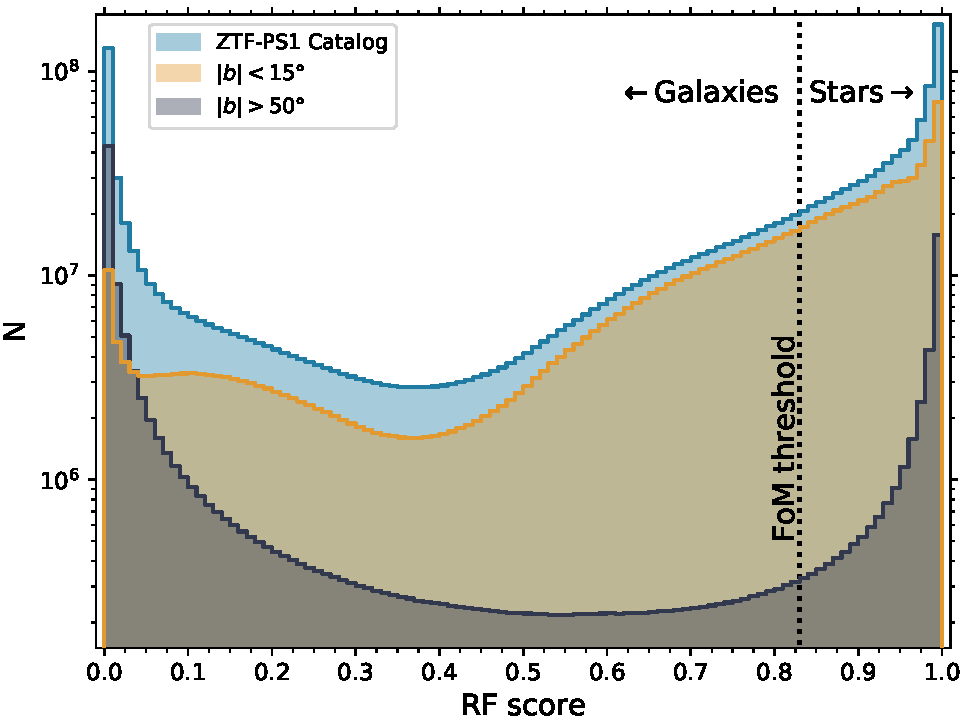
\includegraphics[width=3.35in]{./Figures/ZTF_PS1_cat_hist.pdf}
  %
  \caption{ The distribution of RF classification score for all sources 
 in the ZTF-PS1 star--galaxy
  catalog. Note that the number counts are shown on a log scale. The vertical dotted line shows the FoM-optimized classification threshold, sources to the right of the line are classified as stars. The full catalog is shown in blue, while Galactic plane sources ($|b| <
15^{\circ}$) are shown in orange, and high galactic latitude sources ($|b| > 50^{\circ}$) are shown in grey. Ambiguous classifications ($0.2 \lesssim
\mathrm{RF\;score} \lesssim 0.8$) in the catalog are dominated by sources in the Galactic plane.}
  %
  \label{fig:ztf_hist}
\end{figure}
%%%%%%%%%%%%%

In total, there are 1,484,281,394 sources with classifications in the ZTF
database. A histogram showing the distribution of the final classifications
is shown in Figure~\ref{fig:ztf_hist}. The thresholds appropriate for
identifying point-source counterparts to the ZTF candidates are reported in
Table~\ref{tbl:fpr} (note that these thresholds apply to
$\mathtt{nDetections} \ge 3$ sources). Of the $\sim$1.5$\times 10^{9}$
sources in the ZTF-PS1 catalog, 734,476,355 ($\sim$50\%) are classified as
stars using the FoM-optimized classification threshold of 0.83.

Figure~\ref{fig:ztf_hist} additionally shows that most of the stars in the
catalog are located in the Galactic plane, most of the (high-confidence)
galaxies are outside the plane, and (unsurprisingly) that classification is
more challenging in regions of high stellar density. At high galactic
latitudes ($|b| > 50^{\circ}$), where the distribution of sources is similar
to the \textit{HST} training set, sources are well-segregated (RF score
$\approx$0 or 1), with very few ambiguous classifications ($0.2 \lesssim
\mathrm{RF\;score} \lesssim 0.8$). The Galactic plane region ($|b| <
15^{\circ}$) dominates the ambiguous classifications in the ZTF-PS1 catalog.
We attribute this to a lack of reliable training data in
high-stellar-density regions, and significantly more blending, which results
in point sources appearing extended. Thus, identifying stellar sources in
the plane likely requires a lower threshold than the FoM-optimized
classification value. The final tuning of the star--galaxy classification
thresholds is a critical early step in the filtering of ZTF candidates
(e.g., \citealt{Kasliwal:18:ZTF}), which is necessary to optimize follow-up of newly
discovered transients.


\section{Summary and Conclusions}

We have presented the development of a large ($\sim$1.5$\times 10^{9}$),
deep ($m \lesssim 23.5\,\mathrm{mag}$) catalog of stars and galaxies based
on PS1 data. We classify these stars using a machine-learning framework
built on a RF model. The RF model is trained using 47,093 PS1 sources with
\textit{HST} COSMOS morphological classifications.

To construct the RF model, we introduced ``white flux'' features, which
correspond to a weighted mean of the relevant features over the
$grizy_{\mathrm {PS1}}$ filters in which a source is detected. The ``white
flux'' features allow us to classify all PS1 sources, irrespective of the
filters in which the source was detected or the line-of-sight reddenning.
One of these newly created features, \texttt{whitePSFKronDist}, is useful on
its own for separating stars and galaxies. Unlike a hard cut on the PSF and
Kron flux ratio, as is employed by the SDSS and PS1 models,
\texttt{whitePSFKronDist} retains knowledge of the SNR and therefore can
provide higher confidence classifications. From \texttt{whitePSFKronDist} we
created the simple model, which does a good job of separating stars and
galaxies. Ultimately, the 11 ``white flux'' features, used in combination
with the RF algorithm, provide the best classification of PS1 sources.

CV on the \textit{HST} training set shows that the RF (FoM$ = 0.71$) and
simple (FoM$ = 0.657$) models greatly outperform the PS1 (FoM$ = 0.007$)
model. For faint sources ($\mathtt{whiteKronMag} > 20$\,mag) the PS1 model
misclassifies many galaxies as stars, while both the simple and RF models
provide overall classification accuracies $\gtrsim 85$\% as faint as
$\mathtt{whiteKronMag} = 23$\,mag.

We find that when evaluated with the SDSS test set, the SDSS and PS1 models
provide more accurate classifications than the RF and simple models,
especially for faint ($\mathtt{whiteKronMag} \gtrsim 21$\,mag) sources. This
reversal, relative to the \textit{HST} training set results, can be
attributed to a bias in the SDSS test set and the SDSS classification model.
In the SDSS test set point sources outnumber galaxies at the faint end,
which is counter to what is observed (at high galactic latitudes).
Furthermore, the SDSS and PS1 models, which utilize a hard cut on flux
ratios, are likely to classify low SNR sources as stars. Together, these
effects amplify the perceived performance of the SDSS and PS1 models. Using
a bootstrap resampling procedure, we correct for the relative number counts
bias in the SDSS test set, and find that the RF and simple models outperform
the SDSS and PS1 models, both in terms of FoM and overall accuracy. Thus, of
the 4 models considered in this study the RF model is superior to all others.

We have deployed the RF model in support of the ZTF real-time pipeline,
resulting in the classification of $\sim$1.5$\times 10^{9}$ sources. The
catalog is dominated by stars in the vicinity of the Galactic plane, though
we find that there are more galaxies than stars at high galactic latitudes,
as is expected at the depth of PS1. ZTF is currently producing public alerts
for newly discovered variability, and the ZTF-PS1 catalog is essential for
removing the numerous foreground stellar flares, false positives in the
search for KNe and other fast transients, from the extragalactic alert
stream.

Moving forward, the release of parallax and proper motion measurements for
$> 10^{9}$ compact sources observed by the \textit{Gaia} satellite
\citep{GaiaDR2} will significantly increase the fidelity of the PS1
star--galaxy catalog. The \textit{HST} training set has very few bright
sources and no sources at low Galactic latitudes, leading to less confident
classifications in these regions (see Figure~\ref{fig:ztf_hist}). As a
space-based observatory, \textit{Gaia} will resolve many stellar blends in
the Galactic plane and identify millions of stars brighter than 16\,mag.
Many of the ambiguous classifications in the ZTF-PS1 catalog (see
\S\ref{sec:ztf}) will be directly identified as stars due to their high
proper motions and parallaxes. The addition of \textit{Gaia} will also
present new challenges, however, as the spacecraft does not downlink
measurements for extended sources. Thus, while \textit{Gaia} would allow us
to increase the size of our training set by many orders of magnitude, it
would also introduce a significant class imbalance. Correcting for the lack
of galaxies would require new approaches beyond those described here. It
should also be noted that \textit{Gaia} alone is not sufficient for our
purposes, as it only detects sources with $G \lesssim 21$\,mag, which does
not include the faint, flaring stars that we expect to be the primary false
positive in the search for fast transients. Nevertheless, our ability to now
merge several $\sim$all-sky surveys provides unprecedented power in the
classification astronomical sources. 
\NC{
In addition to the reinforcement of the amount of relevant information for each source, 
the assessment and the use of a machine-learned classifier 
with an alternative ensemble learning algorithm 
(e.g., adaptive boosting algorithm; \citealt{Freund97}) 
would be meaningful to ensure and to strengthen the power of the star--galaxy separation \citep{Sevilla18}. 
}
This power is particularly important
for improving the scientific output and follow-up efficiency of time-domain
surveys.

\acknowledgements

This work would not have been possible without the public release of the PS1
and SDSS data. We are particularly grateful to the MAST PS1 team for
answering several inquiries regarding the PS1 data, and especially B.~Shiao,
who helped us navigate the PS1 database. We thank M.~Graham and A.~Mahabal
for early conversations regarding the training of the RF model, and B.~Bue
for a discussion about cross validation strategies.

Y.T.\ is funded by JSPS KAKENHI Grant Numbers JP16J05742. Y.T.\ studied as a
Global Relay of Observatories Watching Transients Happen (GROWTH) intern at
Caltech during the summer and fall of 2017. GROWTH is funded by the National
Science Foundation under Partnerships for International Research and
Education Grant No 1545949. A.A.M.\ is funded by the Large Synoptic Survey
Telescope Corporation in support of the Data Science Fellowship Program.

\facility{PS1, Sloan}

\software{\texttt{astropy} \citep{Astropy-Collaboration13}, 
          \texttt{scipy} \citep{Jones01}, 
          \texttt{matplotlib} \citep{Hunter07},
          \texttt{pandas} \citep{McKinney10},
          \texttt{scikit-learn} \citep{Pedregosa12}}


% \appendix


\bibliographystyle{aasjournal}
\bibliography{star_gal}

\end{document}